\documentclass[a4paper]{book}
\usepackage[utf8]{inputenc}

\usepackage{geometry}
\usepackage{bookmark,hyperref}
\usepackage{xcolor}
\usepackage[english]{babel}
\usepackage{graphicx}


\usepackage{amsmath}
\usepackage{amsfonts}
\usepackage{amsthm}

\usepackage{mathrsfs}
\usepackage{bbm}
\usepackage{enumitem}
\usepackage{cleveref}
\usepackage{titlesec}
\usepackage{minitoc}
\usepackage{fancyhdr}
\usepackage{ragged2e}
\usepackage{algorithm}
\usepackage{algorithmic}

\usepackage{tikz}
\usetikzlibrary{arrows.meta}

\hypersetup{colorlinks, linkcolor=red, citecolor=blue, urlcolor=blue, bookmarksopen=true, bookmarksopenlevel=0}



% mathbb
\newcommand{\CC}{\mathbb{C}}
\newcommand{\EE}{\mathbb{E}}
\newcommand{\NN}{\mathbb{N}}
\newcommand{\PP}{\mathbb{P}}
\newcommand{\QQ}{\mathbb{Q}}
\newcommand{\RR}{\mathbb{R}}
\newcommand{\VV}{\mathbb{V}}

% mathcal
\newcommand{\cA}{\mathcal{A}}
\newcommand{\cB}{\mathcal{B}}
\newcommand{\cC}{\mathcal{C}}
\newcommand{\cD}{\mathcal{D}}
\newcommand{\cE}{\mathcal{E}}
\newcommand{\cF}{\mathcal{F}}
\newcommand{\cG}{\mathcal{G}}
\newcommand{\cH}{\mathcal{H}}
\newcommand{\cI}{\mathcal{I}}
\newcommand{\cJ}{\mathcal{J}}
\newcommand{\cK}{\mathcal{K}}
\newcommand{\cL}{\mathcal{L}}
\newcommand{\cM}{\mathcal{M}}
\newcommand{\cN}{\mathcal{N}}
\newcommand{\cO}{\mathcal{O}}
\newcommand{\cP}{\mathcal{P}}
\newcommand{\cQ}{\mathcal{Q}}
\newcommand{\cR}{\mathcal{R}}
\newcommand{\cS}{\mathcal{S}}
\newcommand{\cT}{\mathcal{T}}
\newcommand{\cV}{\mathcal{V}}
\newcommand{\cW}{\mathcal{W}}
\newcommand{\cX}{\mathcal{X}}
\newcommand{\cY}{\mathcal{Y}}
\newcommand{\cZ}{\mathcal{Z}}

% mathscr
\newcommand{\sA}{\mathscr{A}}
\newcommand{\sB}{\mathscr{B}}
\newcommand{\sI}{\mathscr{I}}
\newcommand{\sM}{\mathscr{M}}
\newcommand{\sO}{\mathscr{O}}
\newcommand{\sP}{\mathscr{P}}
\newcommand{\sR}{\mathscr{R}}
\newcommand{\sT}{\mathscr{T}}
\newcommand{\sX}{\mathscr{X}}
\newcommand{\sY}{\mathscr{Y}}
\newcommand{\sZ}{\mathscr{Z}}

% \theoremstyle{plain}
% \newtheorem{thm}{Theorem}[chapter]
% \crefname{thm}{theorem}{theorems}
% \newtheorem{prop}{Proposition}[chapter]
% \crefname{prop}{proposition}{propositions}
% \newtheorem{lem}{Lemma}[chapter]
% \crefname{lem}{lemma}{lemmas}
% \newtheorem{cor}{Corollary}[chapter]
% \crefname{cor}{corollary}{corollaries}

% \theoremstyle{definition}
% \newtheorem{defi}{Definition}[chapter]
% \crefname{defi}{definition}{definitions}
% \newtheorem{assu}{Assumption}[chapter]
% \crefname{assu}{assumption}{assumptions}
% \newtheorem{rem}{Remark}[chapter]
% \crefname{rem}{remark}{remarks}
% \newtheorem{ex}{Example}[chapter]
% \crefname{ex}{example}{examples}

% operateurs
\DeclareMathOperator{\Tr}{Tr}
\DeclareMathOperator{\Supp}{Supp}
\DeclareMathOperator{\Vect}{Vect}
\DeclareMathOperator*{\argmin}{arg\,min}
\DeclareMathOperator*{\argmax}{arg\,max}
\DeclareMathOperator{\Cov}{Cov}
\DeclareMathOperator{\Var}{Var}
\DeclareMathOperator{\erf}{erf}
\DeclareMathOperator*{\tend}{\to}
\newcommand{\rD}{\mathrm{D}}
\def\bX{\mathbf{X}}
\DeclareMathOperator{\diag}{diag}
\DeclareMathOperator{\Span}{Span}
\DeclareMathOperator{\Image}{im}
\DeclareMathOperator{\Kernel}{ker}


\newcommand{\conv}[2][\ ]{\overset{#1}{\underset{#2}{\to}}}
\newcommand{\aseq}[2][]{\overset{#1}{\underset{#2}{=}}}
\newcommand{\equi}[1]{\underset{#1}{\sim}}
\newcommand{\mbf}[1]{\mathbf{#1}}
\newcommand{\indic}{\mathbbm{1}}
\newcommand{\hatmbf}[1]{\hat{\mathbf{#1}}}
\let\eps\varepsilon
\let\to\longrightarrow


\newenvironment{abstract}[1][Abstract]{\paragraph{#1}}{}





% \defbibheading{none}{%
% }
% \DeclareSourcemap{
%   \maps[datatype=bibtex]{
%     \map[overwrite]{
%       \perdatasource{biblio.bib}
%       \step[fieldset=keywords, fieldvalue={,conf}, append]
%     }
%   }
% }




\newcommand{\PhDTitle}{%
	%Reference priors: objective and practical inference,applied for auditable estimations of seismic fragility curves\\%
    %
    Extended reference prior theory for objective and practical inference, application to %\makebox[4em][r]
    {robust and auditable seismic fragility curves%}
}}

\newcommand{\logoEd}{EDMH}																		%% Logo de l'école doctorale. Indiquer le sigle (EDIPP, EDMH) / Doctoral school logo. Indicate the acronym : EDMH, EDIPP
\newcommand{\PhDTitleFR}{Théory des priors de référence étendue pour une inférence objective et pratique, application pour des estimateurs auditable de courbes de fragilité sismique}													%% Titre de la thèse en français / Thesis title in french
\newcommand{\keywordsFR}{Prior objectif, Analyse bayésienne, Aléa sismique, Courbe de fragilité, Quantification des incertitudes}														%% Mots clés en français, séprarés par des , / Keywords in french, separated by ,
\newcommand{\abstractFR}{%
La théorie des priors de référence fournit un cadre approprié à une inférence bayésienne objective, puisqu'elle %visant à minimiser
vise à minimiser la subjectivité introduite et à permettre aux informations issues des données d'orienter la distribution des estimations. Pour cette raison, l'application de cette théorie à l'estimation des courbes de fragilité sismique est particulièrement pertinente. En effet, ces courbes
sont des éléments essentiels
des études simsmiques probabilistes de sûreté~; elles expriment la probabilité de défaillance d'une structure mécanique en fonction d'indateurs définissant des scénarios sismiques. Puisqu'elles informent des décisions critiques en matière de sécurité des infrastructures, une auditabilité complète de l'approche qui conduit aux estimations de ces courbes est nécessaire.

Cette thèse étudie l'interaction entre la théorie des priors de référence et l'estimation des courbes de fragilité sismique, apportant des contributions originales dans ces deux domaines. Tout d'abord, nous complétons les fondements théoriques des priors de référence en développant de nouvelles constructions de ceux-ci. Notre objectif est de soutenir leur objectivité tout en améliorant leur applicabilité pratique. Nos résultats prennent la forme de contributions théoriques dans ce domaine qui sont basées sur une définition généralisée de l'information mutuelle. Nos approches abordent les principaux problèmes des priors de référence, à savoir le caractère impropre de leur distribution ou de leu distribution \emph{a posteriori}, et leur formulation complexe pour une utilisation pratique.

Esnuite, nous revisitons l'estimation des courbes de fragilité sismique basée sur le modèle probit-lognormal dans un contexte où les données sont particulièrement rares. Notre objectif est de réaliser une estimation bayésienne des courbes de fragilité qui tire parti de l'optimisation de toutes sortes d'informations, y compris l'information \emph{a priori}, afin de fournir des estimations robustes et auditables. Nos résultats mettent en évidence les limites et les irrégularités du modèle et proposent des méthodes qui fournissent des estimations précises et efficaces des courbes. Les évaluations de nos approches sont réalisées sur différents cas d'étude issus de l'industrie nucléaire.

Cette thèse établit un lien fort entre ces deux domaines. L'application aux courbes de fragilité sismique a non seulement motivé les développements théoriques mais leur a aussi directement profité, produisant finalement un cadre d'estimation plus robuste, interprétable et vérifiable.
}															%% Résumé en français / abstract in french

\newcommand{\PhDTitleEN}{\PhDTitle}													%% Titre de la thèse en anglais / Thesis title in english
\newcommand{\keywordsEN}{Objective prior, Bayesian analysis, Seismic hazard, Fragility curve, Uncertainties quantification}														%% Mots clés en anglais, séprarés par des , / Keywords in english, separated by ,
\newcommand{\abstractEN}{%
Reference prior theory provides a principled framework for objective Bayesian inference, aiming to minimize subjective input and allow data-based information to drive the estimates distribution. %This is particularly valuable in high-stakes applications, where transparency, auditability, and robustness are essential. 
% This theory becomes particularly relevant for
For this reason, the application of this theory to the estimation of seismic fragility curves is particularly relevant.
Indeed, these curves are essential elements of seismic probabilistic risk assessment studies; they express the probability of failure of a mechanical structure as a function of indicators that define 
seismic scenarios. Since they inform critical decisions in infrastructure safety, a complete auditability of the pipeline that leads to the estimates of these curves is required.
% they require a total auditability and robustness of the pipeline that produce estimates of them.

%One such application is the estimation of seismic fragility curves—probabilistic tools that characterize structural failure likelihood as a function of earthquake intensity. These curves play a central role in seismic probabilistic risk assessment, where they inform critical decisions in infrastructure safety and resilience.

This thesis investigates the interplay between reference prior theory and seismic fragility curves estimation, yielding original contributions in these two domains. First, we complement the theoretical foundations of reference priors by developing novel constructions of them. 
Our goal is to support their objectivity while improving their practical applicability. Our results take the form of
theoretical contributions in this domain that are based on a generalized definition of the mutual information.
Our approaches tackle the principal issues of reference priors, namely their improper characteristic or that of their posterior, and their complex formulation for practical use.

%  definition of reference priors
% We tackle the pincipal issues encountered by using the referebce prios in practice by proposing methods that address 
% We provide adaptations of the reference priors definiton
% three theoretical contributions in this domain that propose (i)~an extension of the thoery that supports the objectivity of the Jeffreys prior, (ii)~constraints that can be incorporated to the prior to enhance.
%Our goal is to question the balance between obejctivity
%under constraints, improving their practical applicability, and proposing ways to evaluate and compare their objectivity. 
Second, we revisit the estimation of seismic fragility curves based on the prominent probit-lognormal model in a context where the data are particularly sparse.
Our goal is to conduct a Bayesian estimation of seismic fragility curves that leverages the optimization of every sort of information, including the \emph{a priori} one, in order to provide estimates that are robust and auditable.
Our results highlight the limitations and irregularities of the model and propose methods that provide accurate and efficient estimates of the curves. The evaluations of our approaches are carried out on different case studies taken from the nuclear industry.

%a common yet delicate setting due to data sparsity and binary observations. We formally compute the Jeffreys prior for this model, highlight its limitations, and introduce alternative priors that address issues of degeneracy and inefficiency. We also incorporate optimal experimental design to improve estimation quality.

This thesis builds a strong link between these two domains.
The application to seismic fragility curves not only motivated theoretical developments but also directly benefited them, ultimately producing a more robust, interpretable, and verifiable estimation framework.
%The application to seismic fragility curves not only motivates theoretical developments but also benefits directly from them, yielding estimation pipelines that are more robust, interpretable, and auditable. %Through this bi-directional dialogue, %, we demonstrate how abstract statistical theory can be meaningfully applied to real-world engineering problems.
%we illustrate how reference prior theory can be extended and applied to meet the needs of modern reliability analysis.
}

% \renewcommand{\abstractFR}{\abstractEN}



% The reference prior theory provides the means to define a prior that can be qualified as ``objective''.
% stands as a cornerstone of objective Bayesian analysis. By formally defining priors that aim to minimize the influence of subjective information, it offers a principled framework for drawing inferences that are driven primarily by the observed data. 
% For this reason, the framework of reference prior theory becomes significantly relevant for the estimation of seimsic fragilty curves. Indeed, these curves represent a central component of seismic probabilistic risk assessment studies as they quantify the probability of failure of a mechanical component under a specific seimic scenario. 

% The work developed in this thesis is threefold. First, we make original contributions to the theory of reference priors itself. While the theory has matured significantly since its inception, limitations remain—particularly in its capacity to yield practical and well-behaved priors in complex or constrained settings. We propose new ways to construct and interpret reference priors under conditional constraints, investigate their asymptotic properties, and develop diagnostic tools to compare competing priors in terms of objectivity and robustness. These developments both clarify and extend the mathematical foundations of the theory, paving the way for its application in real-world settings where priors must meet practical requirements.

% Second, we focus on the estimation of seismic fragility curves, specifically under the widely used probit-lognormal model. In this context, observations are typically binary (e.g., structure failed or survived), and data scarcity often undermines the stability of classical estimates. We revisit the estimation problem from a Bayesian perspective, beginning with the formal computation of the Jeffreys prior for this model. We show that, while theoretically objective, this prior exhibits limitations in practice—such as posterior degeneracy in low-information regimes. We respond with methodological innovations, including a new class of constrained reference priors that explicitly address these issues. Furthermore, we explore how experimental design can be integrated into the inferential process to optimally extract information from limited data, significantly improving the robustness and interpretability of fragility estimates.

% Third, and most critically, we bridge the gap between these two domains—using the application to seismic fragility curves as both a proving ground and a source of inspiration for the development of reference prior theory. This bi-directional interplay is a central theme of the thesis. On one hand, the challenges encountered in fragility modeling motivate theoretical advances in the construction and evaluation of priors. On the other, these advances enable new and more reliable methods for estimating fragility curves, especially in data-poor settings. For instance, we demonstrate how sensitivity to prior assumptions can be controlled and quantified within the reference prior framework, enhancing the explainability and auditability of the final risk estimates.

% Taken together, the results of this work not only advance the frontier of objective Bayesian analysis but also deliver tangible improvements to the practice of seismic risk assessment. The integration of these two threads—reference prior theory and fragility curve estimation—offers a powerful example of how abstract statistical ideas can be harnessed to meet concrete engineering needs.
% }															
%% Résumé en anglais / abstract in english




%% Membre n°1 (Président) / Member n°1 (President)
\newcommand{\jurynameA}{Nicolas Bousquet}
\newcommand{\juryadressA}{Professeur, Sorbonne université, LPSM}
\newcommand{\juryroleA}{Rapporteur}

%%% Membre n°2 (Rapporteur) / Member n°2 (Reviewer)
\newcommand{\jurynameB}{Daniel Straub}
\newcommand{\juryadressB}{Professeur, TU Munich, Engineering Risk Analysis Group}
\newcommand{\juryroleB}{Rapporteur}

%%% Membre n°3 (Rapporteur) / Member n°3 (Reviewer)
\newcommand{\jurynameC}{Sophie Ancelet}
\newcommand{\juryadressC}{Ingénieure de recherche, ASNR}
\newcommand{\juryroleC}{Examinatrice}

%%% Membre n°4 (Examinateur) / Member n°4 (Examiner)
\newcommand{\jurynameD}{Julyan Arbel}
\newcommand{\juryadressD}{Chargé de recherche, Inria Grenoble}
\newcommand{\juryroleD}{Examinateur}

%%% Membre n°5 (Directeur de thèse) / Member n°5 (Thesis supervisor)
\newcommand{\jurynameE}{Olivier Le Maître}
\newcommand{\juryadressE}{Directeur de recherche, École polytechnique, CMAP}
\newcommand{\juryroleE}{Examinateur}

\newcommand{\jurynameF}{Mathilde Mougeot}
\newcommand{\juryadressF}{Professeure, ENS Paris-Saclay, Centre Borelli}
\newcommand{\juryroleF}{Examinatrice}

%%% Membre n°6 (Co-directeur de thèse) / Member n°6 (Thesis co-supervisor)
\newcommand{\jurynameG}{Josselin Garnier}
\newcommand{\juryadressG}{Professeur, École polytechnique, CMAP}
\newcommand{\juryroleG}{Directeur de thèse}

%%% Membre n°7 (Invité) / Member n°7 (Guest)
\newcommand{\jurynameH}{Cyril Feau}
\newcommand{\juryadressH}{Ingénieur de recherche, CEA Saclay, SEMT}
\newcommand{\juryroleH}{Encadrant}

%% Membre n°8 (Invité) / Member n°8 (Guest)
\newcommand{\jurynameI}{Clément Gauchy}
\newcommand{\juryadressI}{Ingénieur de recherche, CEA Saclay, SGLS}
\newcommand{\juryroleI}{Invité}

\usepackage[backend=biber, style=authoryear]{biblatex}
\addbibresource{biblio.bib}

\title{Brouillon de manuscrit de thèse}
\author{Antoine Van Biesbroeck}

\begin{document}

\maketitle

\tableofcontents


%\section{}




\newlength{\questlenght}
\settowidth{\questlenght}{\textbf{Question iii}\ \ }
\newlength{\textminusquest}
\setlength{\textminusquest}{\textwidth}
\addtolength{\textminusquest}{-\questlenght}
\newcommand{\ques}[2]{%
\noindent\textbf{Question #1}\hfill
\begin{minipage}[t][25pt][t]{\textminusquest}
    #2
\end{minipage}    
}


\chapter{Introduction}\label{chap:intro-english}


\begin{abstract}
abstract
\end{abstract}

\minitoc


\section{Motivation and positioning of the thesis}






\subsection{Probabilistic risk assessment studies}



\subsection{Uncertainty quantification in probabilistic risk assessment studies}



\subsection{The choice of the prior in Bayesian studies}

\subsection{Motivating prior elicitation research for SPRA studies}



\section{Outline of the manuscript and contributions}

\subsection{Problems statement and organization of the thesis}



\subsection{List of contributions}













\chapter{Introduction en français}\label{chap:intro-french}

\renewcommand{\chaptername}{Chapitre}
\renewcommand{\partname}{Partie}


\begin{abstract}[Résumé]
    Ce chapitre ne diffère du \hyperref[chap:intro-english]{chapitre 1} que par sa rédaction en langue française.
    Dans ce chapitre, nous introduisons et motivons les travaux de recherche qui ont été conduits au court de cette thèse. Les travaux sont motivés
    principalement par le besoin d'évolution des méthodes d'études sismiques probabilistes de sûreté, mais aussi par le manque de réponse qu'apporte l'état-de-l'art à la question du choix du prior en inférence bayésienne.
    Ces problématiques sont détaillées et
    les travaux sont alors introduits comme s'inscrivant dans celles-ci, le tout donnant lieu à une organisation consistante du manuscrit.
    %en introduisant à la fois leur inscription dans le cadre des études sismiques probabilistes de sûreté et dans le
    %
    %D'une part, nous introduisons le cadre des études sismiques probabilistes de dûreté, et 
    % Dans ce chapitre, nous mettons en lumière les différentes problématiques, à la fois issue de qui motivent 
    % Dans ce chapitre, nous introduisons les différents contextes qui motivent l'existence de cette thèse. D
\end{abstract}

\minitoc

\section{Motivation et positionnement de la thèse}

\subsection{Etudes probabilistes de sûreté}
%

\subsubsection{Historique}

Les études probabilistes de sûreté (EPS) désignent un ensemble de méthodes d'analyses techniques qui permettent de quantifier un risque encouru par une installation lorsqu'elle est sujette à un évènement. L'évènement peut être d'origine naturelle comme artificielle, il peut être de provenance interne comme externe ; il peut s'agir d'un séisme, d'une inondation, d'une combinaison de défaillances internes, entre autres.  % (qui peut être d'origine naturelle comme artificielle, qui peut être interne comme externe). 

Faisant suite au premières recommandations de F. R. Farmer (expert sûreté à la UK atomic authority) dans les années 1960 pour la fiabilité des installations nucléaires,
ces méthodes ont pour caractéristique commune l'introduction de la notion d'incertitude dans la qualification de l'évènement, ses phénomènes et ses caractéristiques (on parle alors d'aléa).
%
%Elles ont été introduites par F. R. Farmer dans les années 1960 [], qui plébiscitait cette idée d'étudier la fiabilité des installations nucléaires en prenant en compte l'aspect probabiliste et incertain des évenements auqelles elle est sujette.
%
Leur cadre et leur concept ont été rapidement adoptés et développés aux Etats-Unis (cf. le rapport de la Nuclear Regulatory Commission, \cite{nrc_pra_1983}). En particulier, de nombreuses études sont venues dès 1968 (\cite{cornell_engineering_1968}) 
y inscrire les analyses de fiabilité parasismique, définissant alors le cadre des études sismiques probabilistes de sûreté (SPRA en anglais). %, en particulier en ce qui concerne le cadre de la fiabilité parasismque.



Le séisme représente en effet un facteur de risque remarquable des études de sûreté.
Premièrement, bien que communément caractérisé par sa magnitude et sa distance à la source, son signal est bien plus riche qu'une fonction bivariée et deux séismes de même magnitude et de même source peuvent avoir des caractéristiques (et des conséquences) significativement différentes.
Deuxièmement, puisqu'il touche à la fois tous les éléments aussi bien externes qu'internes à l'installation, il est la potentielle source de conséquences lourdes sur les équipements et structures.
%voir de réactions en chaîne 
%qui atteindraient le ``noyau dur'' de l'installation (défini comme un ensemble d'élements critiques à l'installation). %, impliquant ainsi un coût élevé.
Le coût potentiel des conséquences d'un aléa sismique peut alors être élevé et critique dans le contexte nucléaire, ce qui en fait un évènement d'intérêt majeur et décisif même dans les zones géographiques où il est rare.


%La prise en compte du séisme comme un aléa s'est confronté à la

Aujourd'hui, la prise en compte de l'aléa sismique sous le cadre des études probabilistes de sûreté est une recommandation internationale dans le contexte de l'industrie nucléaire. Leur cadre d'application dans l'industrie nucléaire française est précisé par l'autorité de sûreté nucléaire et de radioprotection (ASNR)\footnote{Anciennement ASN: l'autorité de sûreté nucléaire (ASN), a été unifiée avec l'institut de radioprotection et de sûreté nucléaire (IRSN) le 1\textsuperscript{er} janvier 2025.} dans la règle fondamentale de sûreté (\cite{asn_regle_2002}).









\subsubsection{L'évolution des EPS en France, au CEA, et dans cette thèse}



%Le rôle des études de sûreté d'une manière générale est de produire une quantification du risque d'une installation, d'une marge de fiabilité, et de démontrer son repsect d'un seuil défini par une autorité de régulation.
% Deux visions s'oppose relativement au sujet de l'avolution des méthodes et des conaissances relatives aux études de sûreté.
%Lors de la mise en place de de seuil et de la règle, plusieur point de vue, motivés par plusieurs intérêts peuvent alors se heurter. Il y a d'une part les exploitants, pour qui la notion de robustesse perdure d'elle même, les marges prises sont là pour tenir compte du manque de conaissances, et il y a ceux pour lesquels la robustess est sans cesse remise en question par les avancées des méthodes et des connaissances (\cite{roger_seisme_2020}).



%L'évolutions des méthodes et des conaissances relatives à la sûreté de 
L'évolution des méthodes et des connaissances relatives à la sûreté des installations nucléaires se fait de manière parallèle à l'évolution de la règle et de la norme imposées à celles-ci. 
Sur le sujet de l'aléa sismique, le rapport à l'évolution de la règle et de la méthode (et donc des EPS) oppose différents points de vue, principalement entre le principal exploitant (EDF) et les experts de l'autorité de sûreté (anciennement l'IRSN, maintenant unifié avec l'autorité de sûreté nucléaire devenue l'ASNR). 
Pour le premier, la robustesse de l'installation n'est normalement pas remise en question par l'avancée des connaissances et des méthodes puisque l’incertitude sur celles-ci fait parti des marges prises en comptes à la construction de l'équipement et calculées pour. Le second pense au contraire que la robustesse est une question perpétuelle et que la marge n’est pas pas faite pour être mordue au fil des connaissances qui s’ajoutent (\cite{roger_seisme_2020}). 
% L'évolution des méthodes EPS reste un champ de voies ouverte, pour lequel les approches s'opposent fondamentalement.
%Il est complxe de définir une voie d'évolution des EPS, et il n'y a pas de vision qui fait l'unanimté
L'ASNR se place alors en arbitre dans ce dialogue, entre autre elle définit le ``séisme majoré de sécurité''\footnote{Aujourd'hui plutôt appelé ``séisme noyau dur''.} (il s'agit d'une majoration du spectre du ``séisme maximal historiquement vraisemblable''\footnote{Aujourd'hui plutôt appelé ``séisme de dimensionnement''.}) qui sert de marge de référence dans la démonstration de robustesse parasismique d'un équipement. % la marge de fiablité et séisme maximal à prendre en compte. %En ce qui concerne l'aléa sismique, le dialogue 
%
%Un tel dialogue n'est pas propre à la France, et 


Cet arbitrage est donc à la fois sensible et critique.
L'incident survenu en 2011 à la centrale nucléaire de Fukushima-Daiichi le démontre. L'aléa sismique (qui est la cause du tsunami) de référence
%fixé par le concensus des experts japonais
a été sous-évalué par le consensus des experts japonais, et c'est cette sous-évaluation qui est au final la cause de l'incident (cf. le rapport de l'agence internationale de l'énergie atomique, \cite{iaea_fukushima_2015}).
%En 2011, a eu lieu un incident 
Suite à cet évènement, l'ASNR a pris la décision de majorer d'un facteur 1.5 le séisme majoré de sécurité en France, imposant une démonstration amplifiée de la robustesse des différentes installations par leur exploitant.



%En 2011, à la suite de l'incident à la centrale de Fukushima suite au séisme survenu au large des côtes japonaises, ce dialogue s'est conclut par une imposition de la part de l'autorité de sûreté d'une majoration d'un facteur de 1.5 de ce séisme majoré de sécurité en France. % de la marge de fiabilité sismique des équipements nucléaires en France. 

%Devant le coût induit par 

%Cette différence démontre de la complexité du sujet






% Le séisme ne fait pas exception
% la place des EPS simsique dans cette différence de vision est très marquée puisque l'aléa du séisme reste une quesiton ouverte en soi, la moindre différence de choix de séisme maximim possible peut donner lieu à une ampleur de changement d'un coût très élevé pour l'exploitant



%Les études probabilistes de sureté ont été adoptées progressivement en France 


%En France, l'industrie nucléaire est réduite à un nombre restreint d'acteurs, exploitants, experts indépendants, et autorité.

% Ambivalence de la robustesse, deux notions 
% deux visions
% Le CEA, à la fois exploitatn et expert

La place du CEA est ambivalente dans l'échiquier nucléaire français.
D'une part, il est exploitant d'installations nucléaires de recherche 
et joue alors son propre rôle quant à la démonstration de robustesse de ses équipements.
Aussi,
%, et ausi %titulaire d'une mission d'expertise de sûreté.
il participe à l'expertise conjointe des expertises de sûreté relatives au parc nucléaire civil exploité par EDF. 
%Le CEA joue son propre rôle dans l'évolution de la démonstration de la robustesse de ses propres equipements et installations. 
La recherche et l'expertise sur les causes de l'aléa sismique % études simqiques de sûreté au CEA 
se fait au CEA au laboratoire EMSI, qui dispose d'une plateforme expérimentale (Tamaris) qui permet de procéder à divers tests mécaniques sur des équipements sous séismes. 
%Le laboratoire d'etudes mécaniques et sismiques (EMSI) s'inscrit pleinenemnt dans cette ambivalence. Propriétaire de la plateforme d'expérimentation sismique Tamaris, le labortoire se place souvent au centre des études de fiabilité sismique et du dialogue entre EDF et les experts de l'ASNR.
L'approfondissement des méthodes des études sismiques probabilistes de sûreté est un enjeu du CEA qui s'inscrit dans ce laboratoire. Le CEA étant responsable devant les autorités de sûreté de ses installations, il cherche %alors 
à développer des méthodes toujours rigoureuses devant leur vieillissement. %de ces installations et de leurs équipements.



% Le rôle du CEA est ambivalent dans cete equation, à la fois exploitant instut de recherche.
% Le CEA joue son propre rôle dans l'évolutions de la démonstration de robstesse de ses propres installations. Aussi il participe à l'expertise conjointe de méthodes d'EPS avec EDF.


% Le CEA est lui même exploitant, d'unstallations de recherche.
% Il a 

% L'evolutio des EPS y est toujours un enjeux pour être capable de produire une étude plus efficace, et des résultats plus convaincants aurpès des autorités.
% Le CEA est responsable auprès des autorités concernant ses installations et cherche à développer des méthodes toujours rigoureuses devant le vieillissemnt des installations

% Sur le sujet de l'aléa sismique, la démonstration de robustesse reste complexe vis à vis de la complexité de l'aléa lui-même, et de sa fréquence.
% Les EPS sont en constantes ré-évaluation à la demande des autorités de sûreté sur cette aspect, principalement depuis l'accident sur la centrale de Fukushima en 2011. %%% Peut etre mettre ca plus haut

% Au CEA, la recherche sur les études sismiques probabilistes de sûerté est portée par le laboratoire EMSI, qui dispose d'une plateforme experimentale (Tamaris) qui permet de procéeder à divers tests mécaniques sur des équipements sous séismes. 

Cette thèse s'inscrit dans la démarche d'évolution du SPRA et de démonstration de sûreté. Financée par le CEA dans le cadre d'un contrat de formation par la recherche, elle a pour objectif d'étoffer l'état de l'art en terme d'estimation de fragilité sismique des équipements et des installations.
L'objectif est de développer des méthodes qui doivent le plus possible être (i) efficaces devant la complexité des objets étudiés et de la définition de l'aléa, (ii) être robustes dans le temps et devant une potentielle réévaluation des critères de sûreté, et (iii) être transparentes et auditables par les autorités de sûreté.

%lieu à des méthodes qui savent être efficace devant la complexité technique représentée efficaces devant la c

%en cherchant un cadre plus robuste, plus efficace.
%%%% Principalement en appuyant l'étude bayésienne de celles-ci.




\subsection{La quantification d'incertitudes dans les études probabilistes de sûreté} % la quantification d'incertitutde dans les EPS


\subsubsection{Principe et étapes de la quantification d'incertitudes}

%Le cadre des EPS regroupe un certains nmb
%Différents outils mathématiques sont employés dans le cadre des EPS et composent

Les études probabilistes de sûreté %et plus généralement les études probabilistes de fiabilité, de robustesse, et de  %les procédés de génie probabiliste d'études de fiabilité, de robustesse, et de 
s'appuient sur la 
prise en compte et la quantification des incertitudes qui apparaissent dans le procédé d'évaluation d'un risque au sein d'un système physique.
%lors de l'évaluation d'une quantité décrivant un risque. %d'un 
%
La quantification d'incertitudes représente en fait une démarche qui consiste à modéliser et analyser méthodiquement l'incertitude, sa source, et sa propagation au sein de la modélisation du système physique étudié. %étudié. %système phyisique?
Elle se construit alors à l'intersection de la physique, de l'ingénierie et des mathématiques appliquées, et s'érige même comme une branche des statistiques à part entière.

Elle concentre son étude sur 3 éléments qui décrivent l'interaction entre le système physique et l'aléa : des paramètres d'entrée $\mbf X$, une réponse physique du système $ Y$, et une modélisation de celle-ci selon : $ Y=\cM(\mbf X)$. % ($\cM$ peut-être définit comme la ).
Cette fonction $\cM$ est liée à la modélisation, souvent complexe, du système et de ses propriétés physiques (il peut s'agir de la résolution d'équations physiques, de simulation numériques, ou même du résultat d'une expérience mécanique).
%L'objet de la quantification d'incertitude est alors d'évaluer une quantité d'intérêt qui dépend de $\mbf Y$ : comme une variance, une probabilité de défaillance, etc ; plus généralement une quantité de la forme $\EE\,\phi(\mbf Y)$.
%
La démarche générale de la quantification d'incertitudes est souvent décrite au travers de différentes étapes clés (voir par ex. \cite{sudret_uncertainty_2007, iooss_contributions_2009}), à savoir : %au sein desquelles on distingue particulièrement l'étape d'identification des sources d'incertitudes.
%qu'on peutt principalement résumé 
%
\begin{enumerate}
    \item L'identification des sources incertitudes : 
        il est usuel de classifier les incertitudes selon deux grandes catégories. D'une part les incertitudes irréductibles, qui proviennent du hasard ``naturel'' embarqué dans l'aléa et le système physique. D'autre part, les incertitudes épistémiques, qui existent par manque d'information, et qui sont alors considérées comme réductibles en opposition aux précédentes (\cite{hullermeier_aleatoric_2019}). Il s'en suit une modélisation probabiliste de l'entrée $\mbf X$. 
    \item La propagation des incertitudes : cette étape correspondant à l'approximation de la distribution du modèle $\cM(\mbf X)$, et de l'évaluation d'une quantité d'intérêt qui dépend de celle-ci : comme une variance, une probabilité de défaillance, etc ; plus généralement une quantité de la forme $\EE\,\phi( Y)$.
%     et de celle de la quantité d'intérêt $\phi(\mbf Y)$. %De nombreuses méthodes mathématiques viennent en appui à cette étape, et sont évoquées plus bas.
    \item L'analyse de sensibilité : son rôle est de comprendre avec plus de recul la manière dont l'incertitude se propage dans un système, en identifiant l'impact d'un ou de plusieurs des paramètres d'entrées sur la sortie $ Y$ (\cite{iooss_review_2015}).
    %L'analyse de sensibilité se construit depuis les premier travaux de Sobol' (\cite{sobol_sensitivity_1993})
    %, lorsque les entrées sont multivariées ($X=(X_1,\dots,X_p)$), quelles sont celles  
\end{enumerate}


\subsubsection{Des outils mathématiques en quantification d'incertitudes}

%L'étape 1 sus-mentionnée s'ajoute à la modélisation du  modélisation
%Les étapes 2 et 3 ci-dessus mentionnées 
De nombreux outils mathématiques viennent appuyer les étapes sus-mentionnées. Bien que ce manuscrit n'a pas pour but d'en décrire un panel exhaustif, ci-dessous sont listés quelques exemples qui reviennent dans les travaux de cette thèse.
%en voici quelques uns qui sont omniprésents dans le domaine

\begin{itemize}
    \item La métamodélisation %, %le plus souvent par processus gaussien (appellé aussi krigeage), ou par polynomes du chaos, 
    permet de contrevenir la complexité d'évaluation du modèle $\cM$, en construisant un méta-modèle $\tilde\cM$, entraîné à partir d'une base de données d'observations $(\mbf x_1, y_1),\dots,(\mbf x_k,y_k)$. Le méta-modèle se veut par principe plus simple à évaluer que le modèle réel. 
    Rien ne limite sa définition explicitement qui peut aller d'un simple modèle paramétrique à la sortie d'un réseau de neurones ``boîte noire'' ; parmi les plus commun on peut évoquer la méta-modélisation par processus gaussien (ou krigeage) et par polynômes du chaos. %Dans le cadre d'études de sûreté, on citera par exemple \cite{}
    %
    \item Les indices globaux de sensibilité s'inscrivent pleinement dans l'étape d'analyse de sensibilité du système.
    % 
    Ils constituent depuis les premiers travaux de \citet{sobol_sensitivity_1993} des outils essentiels pour mesurer statistiquement comment $ Y$ est impactée par un ou plusieurs des $X_i$ (où $(X_1,\dots,X_p)=\mbf X$). Dans ce cadre, l'impact, noté $S_i$, de l'entrée $X_i$ sur $ Y$ s'exprime comme une divergence moyenne entre la distribution $\PP_{ Y}$ de $ Y$ et sa distribution conditionnellement à $\mbf X$, $\PP_{Y|\mbf X}$ \citep{da_veiga_global_2015} : 
        \begin{equation}
            S_i = \EE_{X_i}[D(\PP_{ Y}||\PP_{Y|X_i})],
        \end{equation}
    où $D$ est une mesure de dissimilarité entre deux mesures de probabilité.
    Le choix de $D$ est alors décisif dans l'étude de $S_i$. %, qui revient à une étude de divergence entre deux mesures de probabilité. 
    On peut noter, par exemple, que choisir $D$ définie par $D(P||Q) = \|\EE_{X\sim P}X-\EE_{X\sim Q}X\|^2$ revient à étudier un indice de Sobol' du premier ordre.
    Le choix de $D$ peut être motivé par divers intérêts, par exemple, celui de discriminer  l'indépendance entre $X_i$ et $ Y$. Le point suivant détaille un large panel de choix possibles pour $D$.

    \item La théorie de l'information est au centre de la comparaison de mesures de probabilité et donc de la quantification d'incertitudes. Par essence, les manières de comparer la façon qu'ont deux mesures de probabilité de  distribuer l'information dans un espace sont vastes. 
    Dans la définition de $S_i$ plus haut, le choix de $D$ (et donc le choix de définition de $S_i$) relève de la théorie de l'information.
    
    
    % , puisque deux distributions difères par la manière dont elles 
    Un choix alors commun, perçu comme une extension de l'entropie de Shannon, est celui des $f$-divergences de \citet{csiszar_information-type_1967}. On peut noter qu'elles sont employées dans des domaines variés, au-delà de l'analyse de sensibilité, tel que l'inférence variationnelle (\cite{minka_divergence_2005,bach_sum--squares_2023}), le design de méta-modèles (\cite{nguyen_surrogate_2009}), l'apprentissage PAC-bayésien (\cite{picard-weibel_change_2022}).
    Lorsque $f$ est convexe que $f(1)=0$, elle sont définies selon :
        \begin{equation}\label{eq:intro-fdiv-french}
            D_f(P||Q) = \int_\cX f\left( \frac{p(x)}{q(x)} \right) q(x)d\mu(x),
        \end{equation}
    en notant $p$, $q$ des densités associées à $P$ et à $Q$ par rapport à une mesure commune $\mu$ sur leur ensemble de définition $\cX$.     
    Les $f$-divergences réduisent le choix de $D$ à celui de $f$, les plus communément employées étant les $\delta$-divergences (\cite{zhu_information_1995}) définies en fixant $f=f_\delta$ où
        \begin{equation}
            f_\delta(x) = \left\lbrace\begin{array}{l l} \frac{x^\delta-\delta x-(1-\delta)}{\delta(\delta-1)} & \text{si\ }\delta\not\in\{0,1\},\\ 
                x\log x-x+1  & \text{si\ }\delta=1, \\
                -\log x +x -1 & \text{si\ }\delta=0.
            \end{array}\right. 
        \end{equation}    
    Il est remarquable que la peut-être plus connue des mesures de dissimilarité (la divergence de Kullback-Leibler) peut être vu comme un cas particulier des $\delta$-divergences. En effet, rappelons que la divergence de Kullback-Leibler, notée $\text{KL}$, est définie par 
        \begin{equation}
            \text{KL}(Q||P) = \int_\cX\log\left(\frac{q(x)}{p(x)}\right)q(x)d\mu(x)
        \end{equation}
        (en adoptant les même notations qu'en équation \eqref{eq:intro-fdiv-french}), si bien que 
        \begin{equation}
            D_{f_\delta}(P||Q) = \text{KL}(P||Q)\ \text{si\ }\delta=1,\quad D_{f_\delta}(P||Q) = \text{KL}(Q||P)\ \text{si\ }\delta=0.
        \end{equation}

    Bien sûr, il existe aussi de nombreuses mesures de dissimilarité qui ne sont pas des $f$-divergences, à ce titre, les indices de Sobol' du premier ordre évoqués plus haut font offices d'exemple. Un autre exemple notable présenté ici est celui des normes maximales de discrépances (MMD). Soient $P$, $Q$ deux mesures de probabilité définies sur un ensemble $\cX$, et soit $\cH$ un espace de Hilbert à noyau reproduisant (RKHS ; un rappel sur cette notion et ses définitions est proposé en annexe) sur $\cX$,  dont le noyau reproduisant est noté $k:\cX\times\cX\to\CC$. %On peut définir les imbrications moyennes  \cite{gretton_kernel_2012}
    On définit la MMD (\cite{gretton_kernel_2012}) par
        \begin{equation}
            \text{MMD}(\cH;\,P||Q) = \sup_{\substack{f\in\cH\\ \|f\|_\cH\leq1}} |\EE_{X\sim P}f(X) - \EE_{X\sim Q}f(X)|,
        \end{equation}
    ou, dans une forme plus simple :
        \begin{equation}
            \text{MMD}^2(\cH;\,P||Q) = \EE_{X,X'\sim P\otimes P}[k(X,X')] + \EE_{Y,Y'\sim Q\otimes Q}[k(Y,Y')] - 2\EE_{X,Y\sim P\otimes Q}[k(X,Y)].
        \end{equation}
        %
    \item L'analyse bayésienne est un outil incontournable de la quantification d'incertitude, puisqu'elle a pour principe fondamental d'introduire une forme d'incertitude dans un ou plusieurs des paramètres du modèle étudié. 
    L'incertitude incorporée par le cadre bayésien peut prendre diverses formes, et se traduit au travers de la définition de l'\emph{a priori}. 
    La propagation d'incertitudes au travers de ce canevas se quantifie en calculant l'\emph{a posteriori}, à partir d'observations statistiques $(\mbf x_1,y_1),\dots,(\mbf x_k, y_k)$.
    La définition de l'\emph{a priori} est critique, elle prend place dans l'étape d'identification des incertitudes, et se révèle impactante sur l'\emph{a posteriori}, et donc, dans un contexte d'étude probabiliste de sûreté, sur le risque.
    
    Puisque ce dernier outil, qui est en fait un paradigme à lui tout seul, est au centre de cette thèse, la section qui suit lui est pleinement dévouée.
\end{itemize}
















\subsection{Le choix du prior dans les études Bayésiennes}

%L'inférence Bayésienne s'inscrit dans le domaine de l'inféérence statistique.
% ici paradigmes freq bayes et intervalles cred conf


L'analyse bayésienne est une théorie des statistiques qui se construit selon une interprétation des probabilités qui sont vues comme des degrés de plausibilité des évènements, on parle généralement de ``crédibilité''. 
%Comme toute théorie statistique =
Comme toute étude statistique, elle cherche à faire le lien entre des observations statistiques et leur distribution probabiliste. %, avec comme particul identifier la distribution de données observée.
Elle s'appuie sur le théorème de Bayes, en considérant l'inconnue qui permet de définir la distribution des données comme étant aléatoire. Les observations statistiques informent alors la distribution de cette inconnue, ce qui met  à jour le degré de crédibilité attribué à une distribution que suivraient les données par rapport à une autre.


Le raisonnement contraire, dit fréquentiste, considère la probabilité comme une fréquence d'occurrence observable au prix de reproduire l'expérience. Sous ce paradigme, l'inconnue existe, 
et les fréquences données par la répétition de l'expérience sont plus probables selon que l'on considère certaines valeurs de l'inconnue plutôt que d'autres, on parle généralement de ``confiance''.


Au final, il est important de noter que ces deux raisonnements se complètent, voire parfois se confondent suivant les cas, et ils sont loin d'être antinomiques. Dans un contexte pratique, le cas d'étude et ses spécificités peuvent néanmoins orienter le choix de favoriser l'un par rapport à l'autre.

%et c'est alors l'aléatoire observé lors de cette répétition qui traduit la confiance en une distribution pluôt qu'en une autre %de l'observation aléatoire qui définit

Dans cette thèse, on se concentre sur l'analyse bayésienne dans le cadre de l'inférence statistique. Dans ce contexte, une variable d'intérêt $Y\in\cY$ est modélisée selon une distribution paramétrique $\PP_{Y|\theta}$, $\theta\in\Theta$ étant l'inconnue, alors considérée comme étant une variable aléatoire dans le canevas Bayésien.
En toute logique, $\theta$ admet une distribution, que l'on appelle le \textbf{prior}.
Lorsque des réalisations de $Y$ successives et indépendantes conditionnellement à $\theta$ sont observées, le \textbf{posterior} se définit comme la distribution de $\theta$ conditionnellement à ces observations. Une région de crédibilité à un niveau $r$ se définit comme une région de $\Theta$ dont la probabilité selon le posterior est au moins égale à $r$.
On notera que dans ce contexte, divers résultats lient les approches bayésienne et fréquentiste d'estimation de $\theta$. Le théorème de Berstein Von-Mises (voir par ex. \cite{van_der_vaart_asymptotic_1992}) en est un exemple.


Notons $\mbf y = (y_1,\dots,y_k)$ les valeurs observées de $k$ réalisations de $Y$. En supposant que tous ces objets existent et sont bien définis, notons $\pi$ la densité du prior (selon une mesure $\nu$), $\ell(\cdot|\theta)$ les densités de $\PP_{Y|\theta}$ (selon une mesure $\mu$) et  $\ell_k(\mbf y|\theta)=\prod_{i=1}^k\ell(y_i|\theta)$, appelée la vraisemblance du modèle. Alors avec ces notations le théorème de Bayes définit la densité du posterior (par rapport à $\nu$) selon :
    \begin{equation}
        p(\theta|\mbf y) = \frac{\ell_k(\mbf y|\theta)\pi(\theta)}{\int_{\Theta}\ell_k(\mbf y|\theta)\pi(\theta)d\nu(\theta)  }.
    \end{equation}
Cette formule fait le lien entre le prior, le modèle (représenté par la vraisemblance), les données, et le posterior qui traduit la prédiction crédible. Elle permet de schématiser le canevas bayésien comme une chaîne de transmission d'information vers l'\emph{a posteriori}, depuis deux sources : le ``réel'' (les observations) et l'\emph{a priori}. Ce schéma est celui présenté ci-dessous.
    \begin{figure}[h]
        \centering
        \begin{tikzpicture}

            \draw[-{Latex[length=1.5mm]}] (-0.4, 0) -- (.5, 0); % english (0, 0) -- (.9, 0); 
            \draw (-0.4, 0) node[left] {Base de données $\mbf y=(y_i)_{i=1}^k\in\cY^k$}; %english (0,0)
             
            \draw (2.4, 0) node {vraisemblance ${\ell_k(\mbf y|\theta)}$}; %englih (2.5,0)
            
            \draw[-{Latex[length=1.5mm]}] (-0.4, -0.6) -- (0.5, -0.6); % english (0, -0.6) -- (0.9, -0.6); 
            \draw (-0.4,-0.6) node[left] {Paramètre $\theta\in\Theta$}; %english (0,-0.6)
            
            \draw (2.4,-0.6) node {prior $\pi(\theta)$}; % english (2.5,-0.6)

            \draw [-] plot [smooth] coordinates {(4.3,0) (4.6,-0.03) (5.05,-0.27) (5.5,-0.3)};
            \draw [-{Latex[length=1.5mm]}] plot [smooth] coordinates {(4.3,-0.6) (4.6,-0.57) (5.05,-0.33) (5.5,-0.3)};

            \draw (5.7,-0.3) node[right] {posterior $p(\theta|\mbf y)\propto{\ell_k(\mbf y|\theta)}{\pi(\theta)}$};
            
        \end{tikzpicture}
    \end{figure}

%D'une certaine manière

Si l'information issue des données ne pose normalement pas question, c'est l'information \emph{a priori} qui concentre l'attention. Par essence, elle est la source de l'incertitude dans le résultat,  sa construction doit se faire de manière attentive lors de l'étape de modélisation et ne peut être arbitraire. 
%On peut noter également que l'information issue des données passe aussi bien au travers du modèle, tel que la vraisemblance le décrit. Cette modélisation qui est alors au centre 
%Différents auteurs placent aujourd'hui la sélection, la validation et la mise à jour du modèle au centre des études bayésienne, définissant cette démarche comme le worflow bayésien \cite{gelman_bayesian_2020}.
Cependant, la formulation bayésienne lui attribue un impact significatif sur le posterior, particulièrement dans des cas où la taille de la base de données est limitée. Une illustration de ce phénomène est proposée en figure~\ref{fig:intro-differentsposteriors}, où différents priors, en apparence proches, donnent lieu à des posteriors très différents, à partir des même observations.
Bien sûr, le diable est dans les détails, et ici, ce sont les queues de distribution des priors, peu discernables sur l'illustration, qui produisent cette différence. Malgré tout cet exemple questionne, et à juste titre, sur le choix du prior.

\begin{figure}[h]
    \centering
    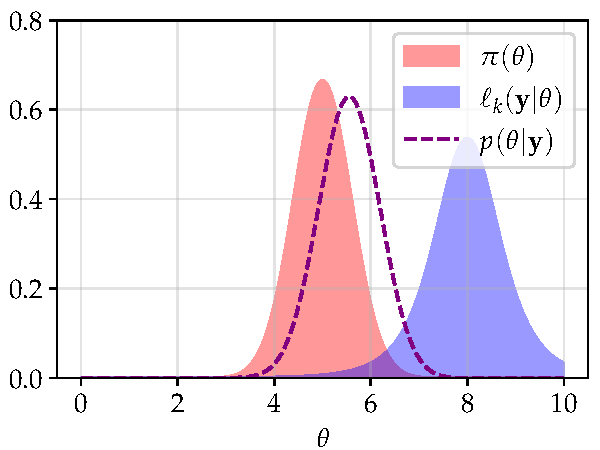
\includegraphics[width=5cm]{figures/intro/posterior1.pdf}
    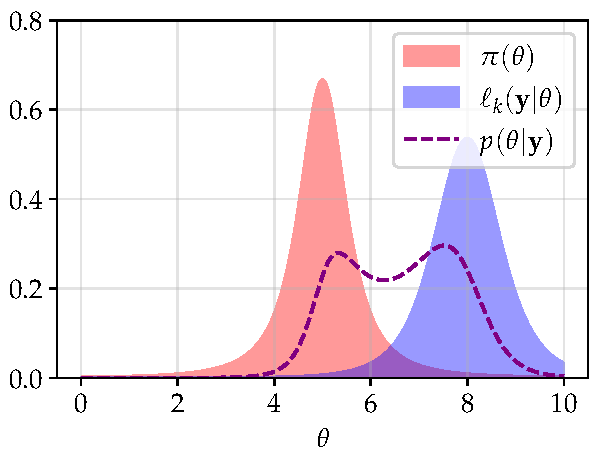
\includegraphics[width=5cm]{figures/intro/posterior2.pdf}
    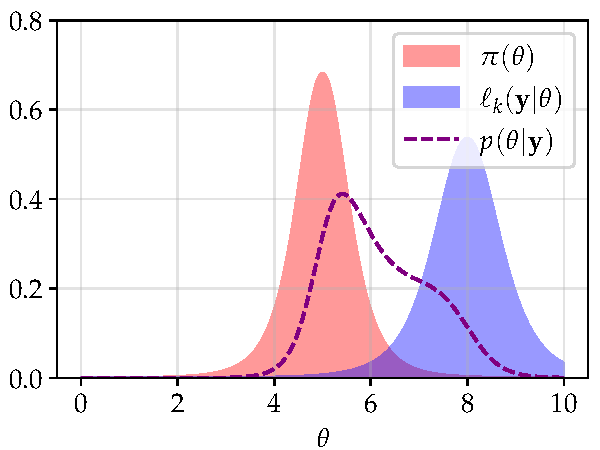
\includegraphics[width=5cm]{figures/intro/posterior3.pdf}   
    \caption{Différents calculs de posteriors (en pointillé) à partir d'une même vraisemblance (bleu) mais de différents priors (rouge).%De gauche à droite le prior est : une gaussienne $\cN(5,)}
    }
    \label{fig:intro-differentsposteriors}
\end{figure}


%On peut déduire d'un tel exemple que les queue de distribution repésente une information décisive au sein d'un prior. Cela illustre 

La question de la construction du prior reste une question ouverte dans la littérature. %tout le worflow bayésien \citep{gelman_bayesian_2020}, elle oppose souvent deux répons%es possibles
%Elle oppose souvent deux axes de refléxions : la définiton de p
Pour certains, elle est l'opportunité d'ajouter de l'information provenant d'une source extérieure, il peut s'agir d'un jugement d'expert, de données historiques, ou de connaissances sur certaines propriétés attendues du résultat. Leurs priors sont plutôt qualifiés d'informatifs.
Pour d'autres, elle est au contraire le moyen d'introduire une incertitude dans le modèle, l'\emph{a priori} est alors dans un tel cas une absence de connaissance, qui vient laisser l'information provenir essentiellement des données. Ces derniers ont confiance en la modélisation de la vraisemblance, et leur prior sera qualifié de non-informatif.


On comprend au travers de ces paragraphes introductifs que cette question est insoluble : il ne peut pas exister de méthode unanime de sélection de prior. Elle illustre même l'un des ``trous'' du workflow bayésien selon \citet{gelman_holes_2020} : les priors trop informés ne permettent pas d'avoir confiance en le moindre résultat tandis que les priors trop peu informés %n'exerguent que trop peu d'estimation crédible.
donnent lieu a des zones de crédibilité parfois trop larges et inutilisables.
%Il ne s'agit pas de décrédibiliser le bayésien 
Ce n'est pas pour autant que l'approche bayésienne perd son intérêt et cette section n'est pas vouée à discréditer la démarche, la suite du manuscrit le prouvera. %Comme toute méthode elle doit être construite 
Mais elle doit laisser celui ou celle qui l'emploie conscient ou consciente des impacts et des limites de ses choix. Le choix d'un prior est aussi critique que le choix du modèle lui-même.








%Lorsque l'on observe plusieurs réalisations de $Y$ sont observées : $(Y_1,\dots,Y_k)$






\subsection{Ce qui motive la recherche sur l'élicitation de priors pour les études sismiques probabilistes de sûreté}

L'analyse bayésienne a gagné en popularité dans de nombreux domaines, y compris dans des études de fiabilité ou de sûreté. 
En effet, elle est plébiscitée pour sa capacité (i) à introduire et propager une incertitude dans un problème d'inférence, et (ii) à être plus régulière que beaucoup de méthodes fréquentistes, en particulier lorsque le nombre de données observées est limité.

Le cadre de l'inférence bayésienne s'introduit en effet bien dans la démarche de quantification d'incertitudes. 
L'identification des incertitudes sur l'entrée $\mbf X$ ou sur le modèle même $\cM$ (ou bien s'il y a lieu le méta-modèle) peut se faire au travers d'une paramétrisation de celles-ci, en donnant lieu à une distribution paramétrique de $Y$ : $\PP_{Y|\mbf X,\theta}$.
La variable $\theta$, aléatoire sous le paradigme bayésien, peut alors représenter diverses sources d'incertitudes, de différentes natures selon les cas \citep{bousquet_contributions_2024}. Cette approche a été employée à pléthore dans divers types de modèles, on peut citer par exemple le cas de processus gaussiens (par ex. \cite{gu_parallel_2016}) ou des réseaux de neurones \citep{arbel_bayes_2023}. 



Parfois, certaines études adoptent la démarche pour la possibilité qu'elle offre d'introduire un jugement  ou une connaissance \emph{a priori}.
C'est pourtant ce même point qui fait aussi débat puisqu'il est la potentielle source d'une subjectivité difficile à justifier.
Dans le cadre des études sismiques probabilistes de sûreté en industrie nucléaire, la démonstration de robustesse est centrale. Les cas d'études y étant souvent très complexes, on trouvera alors parfois autant de priors qu'il y a d'experts en suivant cette démarche.
De tels cas caricaturaux mettent en péril l'auditabilité de la moindre région de crédibilité \emph{a posteriori}.

%De fait, il est essentiel de se chercher à se prévaloir 
%De telles études, compatibles et 
%nécessite l'apport d'un cadre méthodique et rigoureux de 

On comprend en fait que dans une étude de sûreté qui se veut auditable, une ``bonne'' région de crédibilité sur un paramètre estimé n'est pas une région nécessairement étroite, même si elle suggère que la sûreté est satisfaite. A l'inverse, une région trop large n'est pas pour autant ``bonne'' car elle ne permet pas de démontrer la robustesse attendue de l'équipement. L'équilibre est complexe, et le ``bon'' prior est celui qui, bien que démontrant au mieux la capacité ou l'incapacité de l'équipement à résister à l'aléa, produit un résultat inspirant confiance. %Il doit être assuré qu'il est affranchi de l'introduction d

Toutes ces réflexions mettent en lumières l'intérêt d'une construction méthodique du prior dans le cadre des études sismiques probabilistes de sûreté, au travers d'un cadre rigoureux qui évite l'introduction de la moindre subjectivité dans la démarche.










\section{Esquisse du manuscrit et contributions}

\subsection{Problématiques et plan}

% \subsubsection{Problématiques}


Plusieurs questions principales se détachent de cette introduction et de ces premières réflexions. Elles sont listées ci-dessous, et décrivent les problématiques majeures qui se sont manifestées au cours de cette thèse et auxquelles les travaux présentés dans ce manuscrit cherchent à répondre.


\ques{i}{Comment peut-on définir et appuyer l'objectivité d'un prior ?\\ }

\ques{ii}{Quelles sont les limites de l'emploi d'un tel prior, peu informatif par essence, et comment concilier son usage avec les besoins pratiques ?}

\ques{iii}{Comment construire et implémenter de tels priors dans un cas pratique ?\\ }

\ques{iv}{Dans le contexte des études sismiques probabilistes de sûreté, comment s'implémentent ces priors objectifs dans un modèle concret d'estimation de fiabilité sismique ?}

\ques{v}{Quelles conséquences peuvent avoir le manque d'information \emph{a priori} ou provenant des données dans ce modèle et comment les solutionner ?}

\ques{vi}{Comment peut-on finalement bénéficier au mieux des différentes sources d'information dans le workflow bayésien du modèle étudié dans son ensemble ?}\\


Dans cette thèse, nous tentons de répondre à ces six problématiques au travers d'une étude selon deux axes. Le premier axe a une dimension qualifiée de théorique, en adressant les problématiques liées à la construction de prior dits ``objectifs'' dans son ensemble. Il se concentre sur le développement d'une théorie appelée la théorie des priors de référence. Le second axe est alors plutôt qualifié de pratique, en étudiant la mise en œuvre des développements théoriques sur des cas d'études réels, en se concentrant sur l'estimation de courbes de fragilité sismiques, qui représentent un outil important du cadre des études sismiques probabilistes de sûreté.
Il reste important de rappeler que, bien qu'indépendants, les deux grands axes de travail sus-mentionnés s'alimentent l'un l'autre. Ce sont autant les problématiques pratiques qui ont motivé les recherches théoriques, que les découvertes pratiques qui ont permis les études pratiques.\\


%l'un étant plutôt théorique et adresse les questions de construction, de définiton, et d'objectivité des priors ; l'autre étant plut
% Ainsi, la premère partie de ce manuscrit est 




La \textbf{\cref{part:ref-theory}} de ce manuscrit est alors dévouée au développement de la théorie des priors de référence.

\noindent
Dans le \cref{chap:intro-ref}, on introduit la théorie et on développe son état-de-l'art. Il permet d'introduire la notion de prior de référence telle qu'elle est communément définie dans la littérature, et leur place parmi les priors objectifs. Ce chapitre permet aussi de formaliser le cadre mathématique de travail pour la suite de la partie.

\noindent
Dans le \cref{chap:ref-generalized}, on observe que la définition des priors de référence s'appuie sur une mesure de dissimilarité. On cherche alors dans ce chapitre à généraliser la définition de cette dernière afin d'appuyer le caractère objectif des priors de référence. Ce chapitre apporte une réponse à la \textbf{question i}.

\noindent
Dans le \cref{chap:constrained-prior}, on cherche une ouverture au cadre des priors de référence, lorsqu'il donne lieu à des priors difficilement utilisables en pratique. On propose alors une définition de ce qu'on appelle priors de référence contraints. Les solutions de cette définition apportent une réponse à la \textbf{question ii}.

\noindent
Dans le \cref{chap:varp}, on développe une méthode numérique d'approximation des priors de référence. Cette méthode s'appuie sur l'inférence variationnelle en définissant le prior comme la sortie d'un réseau de neurones, afin d'éviter un calcul explicite de celui-ci. Ce chapitre apporte une réponse à la \textbf{question iii}. \\


La \textbf{\cref{part:spra}} de ce manuscrit aborde le sujet de l'estimation bayésienne dite objective des courbes de fragilité sismiques.

\noindent
Dans le \cref{chap:frags-intro}, on introduit les courbes de fragilité sismiques, leur définition, leur historique et leur intégration dans le cadre des études sismiques probabilistes de sûreté. Un état-de-l'art des méthodes d'estimation de ces courbes suivant les différents types de données à disposition y est proposé.

\noindent
Dans le \cref{chap:prem}, on propose un calcul et une étude en profondeur du prior de référence pour un modèle classique employé pour l'estimation de ces courbes de fragilité. L'inférence bayésienne via l'emploi de ce prior y est comparé à d'autres méthodes. Ce chapitre apporte une réponse à la \textbf{question iv}.

\noindent
Dans le \cref{chap:constrained-frags}, on s'intéresse en profondeur aux limites du modèle considéré pour l'estimation des courbes de fragilité. On propose une solution qui est appuyée par les développements théoriques de la première partie. Ce chapitre apporte une réponse à la \textbf{question v}.

\noindent
Dans le \cref{chap:doe}, on termine notre étude en proposant une méthode qui vient appuyer l'estimation bayésienne en optimisant l'information issue des données non plus seulement  lors du choix du prior mais également lors de la sélection de celles-ci, au travers d'une méthode de planification d'expériences. Ce chapitre apporte une réponse à la \textbf{question vi}.\\


Une conclusion générale viendra clore le manuscrit dans une \textbf{\cref{part:conclusion}} finale.


\subsection{Liste des contributions}

La recherche conduite au cours de cette thèse a donné lieu à plusieurs contributions dans la littérature scientifique. Ci après sont listés les travaux publiés pendant celle-ci.

\nocite{van_biesbroeck_design_2024,van_biesbroeck_generalized_2024,van_biesbroeck_influence_2023,van_biesbroeck_properly_2024,van_biesbroeck_reference_2024,baillie_variational_2025}

\begin{itemize}
    \item \textbf{A. Van Biesbroeck}, C. Feau \& J. Garnier (2025). ``Design of experiments for efficient and conform Bayesian learning of seismic fragility curves''. \emph{Proceedings of the 28th conference on Structural Mechanics in Reactor Techology (SMiRT).}
    \item N. Baillie, \textbf{A. Van Biesbroeck}, C. Feau \& C. Gauchy (2025). ``Bayesian estimation of seismic fragility curves based on variational reference priors using neural networks''. \emph{Proceedings of the 6th Thematic Conference on Uncertainty Quantification in Computational Sciences and Engineering (UNCECOMP)}.
    \item \textbf{A. Van Biesbroeck}, C. Gauchy, C. Feau \& J. Garnier (2025). ``Robust a posteriori estimation of probit-lognormal seismic fragility curves via sequential design of experiments and constrained reference prior''. \emph{arXiv} 2503.07343. \textsc{doi:} \href{https://dx.doi.org/10.48550/arXiv.2503.07343}{10.48550/arXiv.2503.07343}.
    \item N. Baillie, \textbf{A. Van Biesbroeck} \& C. Gauchy (2025). ``Variational inference for approximate reference priors using neural networks''. \emph{arXiv} 2502.02364. \textsc{doi:} \href{https://dx.doi.org/10.48550/arXiv.2502.02364}{10.48550/arXiv.2502.02364}
    \item \textbf{A. Van Biesbroeck} (2024). ``Properly constrained reference priors decay rates for efficient and robust posterior inference'', \emph{arXiv} 2409.13041. \textsc{doi:} \href{https://dx.doi.org/10.48550/arXiv.2409.13041}{10.48550/arXiv.2409.13041}
    \item \textbf{A. Van Biesbroeck}, C. Gauchy, C. Feau \& J. Garnier (2025). ``Design of experiments based on a low fidelity model for seismic fragility curves estimation''. \emph{ESAIM: ProcS} (to appear). \textsc{hal:} \href{https://hal.science/hal-04719458v1}{hal-04719458v1}
    \item \textbf{A. Van Biesbroeck} (2023). ``Generalized mutual information and their reference priors under Csizar f-divergence''. \emph{arXiv} 2310.10530. \textsc{doi:} \href{https://dx.doi.org/10.48550/arXiv.2310.10530}{10.48550/arXiv.2310.10530}
    % \item C. Gauchy, \textbf{A. Van Biesbroeck}, C. Feau \& J. Garnier (2023). ``Inférence variationelle de lois a priori de référence''. \emph{Proceedings des 54èmes Journées de Statistiques (JdS)}. \textsc{url}
    \item \textbf{A. Van Biesbroeck}, C. Gauchy, J. Garnier \& C. Feau (2023). ``Connections between reference prior theory and global sensitivity analysis, an illustration with f-divergences''. \emph{Proceedings des 54èmes Journées de Statistiques (JdS)}. \textsc{hal:} \href{https://hal.science/hal-04171446}{hal-04171446}
    \item \textbf{A. Van Biesbroeck}, C. Gauchy, C. Feau \& J. Garnier (2023). ``Influence of the choice of the seismic intensity measure on fragility curves estimation in a Bayesian framework based on reference prior''. \emph{Proceedings of the 5th Thematic Conference on Uncertainty Quantification in Computational Sciences and Engineering (UNCECOMP)}, pp. 94-111. \textsc{doi:} \href{https://dx.doi.org/10.7712/120223.10327.19899}{10.7712/120223.10327.19899}
    \item \textbf{A. Van Biesbroeck}, C. Gauchy, C. Feau \& J. Garnier (2024). ``Reference prior for Bayesian estimation of seismic fragility curves''. \emph{Probabilistic Engineering Mechanics}, 76, pp 103622. \textsc{doi:} \href{https://dx.doi.org/10.1016/j.probengmech.2024.103622}{10.1016/j.probengmech.2024.103622}
\end{itemize}





















%Pour répondre à ces problématiques, 



  % What are the ways to define objectively a prior? Are they totally objective? Are the objective priors the most intersting priors to consider, or should we discriminate judiciously some class of priors? How to compute and implement the objective priors? 
    % What does they look like in the context of SPRA? How to use them in that context and what are the obstacles of the Bayesian approach in the context? 










\newpage
\renewcommand{\chaptername}{Chapter}
\renewcommand{\partname}{Part}



\part{Contribution to the reference prior theory}


\chapter{Review of the reference prior theory}





\section{Introduction}

\section{The standard Bayesian framework}

\section{Prior elicitation: an open literature}

\subsection{Examples, methods, motivations}

\subsection{Informative or non-informative priors? Objective priors and mutual information}


\subsection{Limitations of the State-of-the-art}

\section{A framework for Bayesian inference with improper priors}

\subsection{Definitions and concepts}


\subsection{The reference prior theory in the appropriate framework, review of the definitions and the properties of the reference priors}



%\section{The concept of objective priors and the role of mutual information}

%\section{Reference prior definition and properties}


\section{Open paths and conclusion}


This section should conclude the state-of-the-art and delimit the limitations of the current theory on different aspects. 














\chapter{Generalized mutual information and their reference priors}


\section{Introduction and motivations}


\section{Generalized mutual information}

\subsection{Definitions and developments}

\subsection{Motivating $f$-divergences}


\section{Generalized reference priors}

\subsection{Definitions}

\subsection{Results when $\delta<0$}

\subsection{Results when $\delta>0$}


\section{Discussions}

    \subsection{About the assumptions and their limitations}


    \subsection{About the robustness of Jeffreys prior with different divergences}


        \subsubsection{When $\delta=0$}

        \subsubsection{A heuristic for other $f$-divergences}

        \subsubsection{A simple development with a Maximum Mean Discrepancy divergence}

\section{Conclusion and prospects}
















\chapter{Properly constrained generalized reference priors}



\begin{abstract}[\hspace*{-10pt}]
    This chapter draws mainly on the submitted work: \fullcite{van_biesbroeck_properly_2024}  % Ce chapitre reprend principalement les travaux publiés dans: 
\end{abstract}

\begin{abstract}
    Reference priors are widely recognized for their objective nature. Yet, they often lead to intractable and improper priors, which complicates their application.
Besides, informed prior elicitation methods are penalized by the subjectivity of the choices they require. %to be made.
In this chapter, we aim at proposing a reconciliation of the aforementioned aspects. Leveraging the objective aspect of reference prior theory, we introduce two strategies of constraint incorporation to build tractable reference priors.
One provides a simple and easy-to-compute solution when the improper aspect is not questioned, and the other introduces constraints to ensure the reference prior is proper, or it provides proper posterior.
Our methodology emphasizes the central role of Jeffreys prior decay rates in this process, and the practical applicability of our results is demonstrated using an example taken from the literature.
\end{abstract}

\minitoc



\section{Introduction}\label{sec:BA:intro}


The reference prior theory represents a widely elected theory for constructing priors that are qualified as ``objective''.
The theory has been thoroughly introduced in the \cref{chap:intro-ref}. %It defines priors that maximize the impact of the observed data over themselves in the posterior definition.
The theory provides a formal mechanism to incorporate prior information in a way that maximizes the information gained from the data within the issued \emph{a posteriori} quantities.
In opposition with a plethora of existing  methods for building a prior (see e.g. \cite{mikkola_prior_2023}), 
this process is tuned to prevent the incorporation of subjective beliefs in the workflow.


However, despite their  objective nature,  their implementation is often cumbersome and not always recommended in high dimensions \citep{berger_overall_2015}. %Moreover, 
Moreover, the low-informative nature of these priors is associated with their common improper aspect, necessitating careful handling to ensure valid statistical inference.
Thus, the construction of priors is expected to strike a balance between several criteria. While many works restrict their sets of priors to ones that are tractable, proper, or suitable for high dimensions, others seek to minimize any source of subjectivity.

This chapter aims to reconcile all these criteria to improve the prior elicitation.
Our contribution takes the form of an enrichment of the reference prior theory to leverage the objective aspect that it provides to reference priors. Building on the developments presented in \cref{chap:ref-generalized},
we restrict priors to the ones that belong to  well-chosen ---and not too restrictive--- sets, and we introduce two strategies to define  convenient reference priors.
% First 
Our first strategy provides a simple,  tractable solution for constraining reference priors when the improper aspect is not questioned. The second, by contrast, introduces constraints that lead to  reference priors that are proper, or lead to proper posteriors. 
% 
For both strategies, we try to define the potential loss of objectivity induced by the constraints and we discuss their limits.
Our results emphasize the central role of Jeffreys prior decay rates when they are improper.
Additionally, we draw attention to the fact that our methodology opens a way to define various reference priors on the basis of constraints that could result from any other motivation.



This chapter is organized as follows.
In \cref{sec:BA:defsnotsmots}, after reviewing briefly the notations for the generalized reference priors framework, we develop our motivation and the objective of this work. This section is also the occasion to introduce a novel definition that is useful for the rest of the study: the quasi $D$-reference priors.
Our main results on constrained reference priors are presented in \cref{sec:BA:ress}, and discussed in \cref{sec:BA:discu}.
Then, the  practical aspect of our work is studied by the application of our method to an example taken from  the literature in \cref{sec:BA:exa}. Detailed mathematical proofs are compiled in \cref{sec:BA:proofs}. \Cref{sec:BA:conclusion} terminates the chapter with a conclusion.


\section{Definitions, notations and motivation}\label{sec:BA:defsnotsmots}

\subsection{Notations}\label{sec:BA:nots}

% \subsection{}

% notations IM, results of preceeding chapters, quasi-reference priors

%motivations %maybe its whole section

    %\subsection{The limitations of Jeffreys prior}

    %\subsection{}

In this work we consider a statistic model characterized by a collection of probability distributions $(\PP_{Y|\theta})_{\theta\in\Theta}$ on  a measurable set $(\cY,\sY)$. 
We consider the same construction of the Bayesian framework as in the \cref{chap:intro-ref} (\cref{sec:intro-refs:limits}): considering any prior $\varPi$ (that is a $\sigma$-finite measure on $\Theta$) we denote $\mbf Y_k$ a random vector of $k$ observations whose distribution conditionally to $T=\theta$ is $\PP_{\mbf Y^k|\theta}=\PP_{Y|\theta}^{\otimes k}$, where $T$ is an r.v. whose distribution is the prior $\varPi$.

The modeling is supposed to be regular: we assume $\Theta\subset\RR^d$ with $\nu$ being the Lebesgue measure on $\RR^d$ and every prior $\varPi$ is supposed to admit a density $\pi$ w.r.t. $\nu$ (i.e. $\varPi\in\sM^\nu$).
We also assume that the model admits a likelihood, denoted by $\ell$ with for any $\theta\in\Theta$ and $\mbf y\in\cY^k$, $\ell_k(\mbf y|\theta):= \prod_{i=1}^k\ell(\mbf y|\theta)$. We suppose that it verifies \cref{assu:intro-ref:jeffreysexist} in \cref{chap:intro-ref}, making the Fisher information matrix (denoted $\cI$) and the Jeffreys prior (whose density is denoted $J$) being well-defined.
The marginal distribution (resp. density)  is denoted by $\PP_{\mbf Y_k}$ (resp. $p_{\mbf Y_k}$) and the posterior distribution (resp. density) given the observations $\mbf y\in\cY^k$ is denoted by $\PP_{T|\mbf y}$ (resp. $p(\cdot|\mbf y)$).



Given these notations, we recall the expression of the generalized mutual information, defined in the \cref{chap:ref-generalized}:
\begin{equation}
    \sI_D^k(\varPi) := \EE_{T\sim\varPi}[D(\PP_{\mbf Y_k}||\PP_{\mbf Y_k|T} )],
\end{equation}
with $D$ being a dissimilarity measure.
In this chapter, we mostly focus on such generalized mutual information when $D$ is a $\delta$ divergence with $\delta\in(0,1)$. For some $\delta\in(0,1)$, the notation $D_\delta$ will refer to the $\delta$-divergence whose expression is reminded below:
    \begin{equation}
        D_\delta(P||Q) = \int_\cX f_\delta\left( \frac{p(x)}{q(x)}  \right) q(x) d\omega(x)\quad \text{with}\quad f_\delta(x) = \frac{x^\delta-\delta x-(1-\delta)}{\delta(1-\delta)},
    \end{equation}
where $p,q$ respectively are densities pf $P$ and $Q$ w.r.t. a common measure $\omega$ on $\cX$.
When evoking reference priors in a general way, we will refer to generalized reference priors, as proposed in the \cref{chap:ref-generalized}.
We remind below their definition:
\begin{defi}[Generalized reference prior]\label{def:BA:genref}
    Let $D$ be a dissimilarity measure and $\cP$ a set of priors on $\Theta$. A prior $\varPi\in\cP$ is called a $D$-reference prior over $\cP$ with rate $\varphi(k)$ if there exists an openly increasing  sequence of compact subsets $(\Theta_i)_{i\in\NN}$
    such that $\bigcup_{i\in\NN}\Theta_i=\Theta$ and for any $i$: $0<\varPi(\Theta_i)<\infty $ and
    % with $\pi^\ast(\Theta_i)>0$, $\Theta_i\subset\Theta$, $\bigcup_{i\in I}\Theta_i=\Theta$ such that
        \begin{equation} %\label{eq:defrefpriorsi}
            \lim_{k\rightarrow\infty}\varphi(k)[\sI^k_D(\varPi(\cdot|\Theta_i))-\sI^k_D(P(\cdot|\Theta_i))] \geq0 \text{\ for all\ } P\in\cP\text{\ verifying\ }0<P(\Theta_i)<\infty;
        \end{equation}
    where  $\varphi(k)$ is a {positive and}  monotonous function of $k$. It is said to be unique if for any other $D$-refernce prior $\varPi'$, $\varPi\simeq\varPi'$.
\end{defi}

We also remind the following result on the $D_\delta$-mutual information and their reference priors (see \cref{chap:ref-generalized}).
%  that are defined considering a generalized ,
\begin{thm}\label{thm:BA:l(pi)}
    Suppose $\Theta$ to be compact and $\varPi\in\sM^\nu_\cC$ be a prior with $\varPi(\Theta)=1$. the $D_\delta$-mutual information admits a limit:
        \begin{equation}
            \lim_{k\rightarrow\infty} k^{d\delta/2} \sI_{D_\delta}(\varPi) = l(\pi) - (\delta(1-\delta))^{-1}, \quad l(\pi) = C_\delta \int_{\Theta}\pi(\theta)^{1+\delta} |\cI(\theta)|^{-\delta/2}  d\theta ,
        \end{equation}
        where $\pi$ is the density of $\varPi$, and with $C_\delta= (2\pi)^{d\delta/2} (1-\delta)^{-d/2}/(\delta(\delta-1))$.\\
    Call $\cR\subset\sR_{\cC^b}$ a set of densities such that $M(\cR)=\cP$, with $M$ mapping a density to its associated prior. Then
        $\varPi$ is a $D_\delta$-reference prior over $\cP$ iff $\pi$ maximizes $l$ over $\cR$. 
\end{thm}




\subsection{Objective and motivation}\label{sec:BA:mots}



We already know that the definition of the reference prior and the $D_\delta$-reference prior is satisfied by the Jeffreys prior over the large set of priors $\sM^\nu_\cC$ in most cases (see \cref{chap:intro-ref,chap:ref-generalized}).
% in most case (see \cref{chap:intro-ref} for ). 

%the large set of priors admitting locally bounded and a.e. continuous densities w.r.t. the Lebesgue measure \citep{VanBiesbroeckBA2023}. 

This result is, however, limiting and disappointing in some cases. The reasons are the following ones: (i) the Jeffreys prior is not recommended in high-dimensional problems as it is known to be ``either too diffuse or too concentrated'' \citep{berger_overall_2015}; moreover (ii) when the expression of the likelihood is itself complex, the computation of the Jeffreys prior can become  intractable; %which is why (iii) in practice a restriction to the set of priors to ones which are easier to compute is often favored; 
also (iii) the Jeffreys prior is known to often lead to an improper prior, which does not necessarily issue a proper posterior distribution, essential for practical \emph{a posteriori} inference and sampling.

To tackle these limitations, we propose in this work to restrict the set of priors over which we derive the reference priors.
Indeed, the reference prior definition is usually considered with very large sets of priors, which are constrained only by some regularity assumptions imposed to the priors (such as continuity, positivity). These regularity assumptions do not generally discriminate the Jeffreys prior from the studied set of priors.
In this chapter, different restricted sets of priors will be suggested, they are sets that are though 
to counter the limitations (ii) and (iii) aforementioned. In most cases, they will not include the Jeffreys prior.
%to not include the Jeffreys prior when 



The tackling of limitation (i) mentioned above is not a purpose of this work. We recall that it is actually frequently tackled a sequential construction of the reference prior as %presented in \cref{chap:intro-ref} (\cref{sec:intro-ref:refpriors}).
suggested by \citet{bernardo_reference_1979}.
On the condition that an ordering of the parameters is set:
 \begin{equation}
     \theta = (\theta_1,\dots,\theta_r) \in \Theta=\Theta_1\times\dots\times\Theta_r,
 \end{equation}
this construction considers a hierarchical construction of the reference prior.
It is already described in \cref{chap:intro-ref} (\cref{sec:intro-ref:refpriors}). We remind below the steps of the sequential construction:
%
%Typically, it is recommended to assume $\Theta_j\subset\RR^{d_j}$ with small dimensions $d_j$ (e.g., lower or equal than $2$) for any $j\in\{1,\dots,r\}$, and to sequentially build a reference prior on the $\Theta_j$,  $j\in\{1,\dots,r\}$:
 \begin{enumerate}
     \item initially fix $\ell_k^1=\ell_k$;
     \item for any values of $\theta_{j+1},\dots,\theta_r\in\Theta_{j+1}\times\dots\times\Theta_r$, compute a reference prior (in the sense of \cref{def:intro-ref:ref-priors})  under the model with likelihood $\theta_j\mapsto\ell_k^j(\mbf y|\theta_j,\dots,\theta_r)$, denote $\pi_j(\cdot|\theta_{j+1},\dots,\theta_r)$ its normalized density;
     \item derive $\ell_k^{j+1}$ such as 
         \begin{equation} %\label{eq:hier:condlikeint}
            \ell_k^{j+1}(\mbf y|\theta_{j+1},\dots,\theta_r) =  \int_{\Theta_j}\ell_k^j(\mbf y|\theta_j,\dots,\theta_r)d\pi_j(\theta_j|\theta_{j+1},\dots,\theta_r).
         \end{equation}
 \end{enumerate}

In this work, the reference priors will be derived only given their formal definition (\cref{def:BA:genref}). Yet, our results can be incorporated in this sequential construction. Indeed,
step 2 of the method depicted above consists of the derivation of a reference prior w.r.t. the variable $\theta_j$.
%in the sense of 
% Thus, our reference priors over constrained setes of priors can be  plainly incorporated into this method.
Additionally, we invite to note that this construction does not solve the limitations (ii) and (iii) previously evoked. Actually, it makes them essential. Indeed, step 2 requires, firstly, a derivation of a reference prior, so that it would lead to a low-dimensional Jeffreys prior if the set of priors is not constrained. Also step 3 necessitates, secondly, that the latter leads to a proper posterior so that the integral involved does not diverge.

We note that this last issue is taken into account by \citet{berger_development_1992} with the suggestion of such construction on an increasing sequence of compact subsets of $\Theta$: $\bigcup_{i\in\NN}\Theta_i=\Theta$. The hierarchical reference prior can then be chosen as a limit of the ones obtained under $\Theta_i$ when $i\to\infty$. However, this limit can be cumbersome to derive in practice. Another solution suggested by \citet{mure_objective_2018} is to restrict the $\sigma$-algebra $\sY$ until the reference prior derived in step 2 leads to a proper posterior. It is still imperfect, as there is no guarantee that such a restricted $\sigma$-algebra exists outside the trivial one.


%In the following subsections, we propose a range of solutions to some of the issues aforementioned, based on the derivation of reference priors over constrained setes of priors. In  Section  {sec:constrainedasympt}, we derive a quasi $D_\delta$-reference prior over setes of priors that are easy to compute, in order to tackle the limitations (ii) and (iii) previously evoked. Then, Section  {sec:constrainedproper} explores another kind of constrained setes of priors, which leads to $D_\delta$-reference priors that can solve the item (iv).












\subsection{A useful definition: quasi-reference priors}\label{sec:BA:defsquas}

%As explained in the introduction, the objective of this work is to study reference priors over restricted sets of priors. Indeed, the reference prior definition is usually considered with very large sets of priors, which are constrained only by some regularity assumptions imposed to the priors (such as continuity, positivity). %This regularity does not generally discriminate the Jeffreys prior
%Actually, 
%The choice of the set of priors $\cP$ in \cref{def:BA:genref} remains open and can be restrained from the large one of priors in $\cM^\varrho_\cC/\!\simeq$. %admitting continuous densities w.r.t. the Lebesgue measure.

While we aim at restricting the set of priors $\cP$ in \cref{def:BA:genref}, we must notice
that such a restriction leaves really unsure the existence of a reference prior. 
Indeed, the definition is itself restrictive, as to admit a reference prior, the set $\cP$ must contain a prior whose restrictions are optimal on any compact subsets of $\Theta$.
In this section, we suggest an extension of the definition of reference priors in the case where in the set $\cP$, the optimal priors on compact subsets of $\Theta$ are not renormalization of each other, but converge to a  prior in $\cP$. 
Such convergence is considered in the sense of the Q-vague convergence \citep{bioche_approximation_2016} on $\sM^\nu_\cC$. % on $\cM^\nu\cC/\!\simeq$. This convergence defines a topology 
The Q-vague convergence of a sequence $(\varPi_n)_n$ to a limit $\varPi$ is equivalent to the convergence of $([\varPi_n])_n$ to $[\varPi]$ in $\sM^\nu_\cC/\!\simeq$ for the quotient topology of the vague convergence on $\sM^\nu_\cC$.




\begin{defi}[Quasi reference prior]\label{defi:quasiRefprior}
    Let $\cP$ be a set of priors. We call $\varPi\in\cP$ a quasi $D$-reference prior if it exists an openly increasing sequence $(\Theta_i)_{i\in \NN}$  of compact sets with $\bigcup_{i\in\NN}\Theta_i=\Theta$ such that
    \begin{itemize}
        \item[(i)] for any $i\in \NN$, there exists a $D$-reference prior $\varPi_i$ over $\cP_i=\{P(\cdot|\Theta_i),\, P\in\cP,\,P(\Theta_i)\in(0,\infty) \}$, %, the set of renormalized restrictions to $\Theta_i$ of priors in $\cP$,
        \item[(ii)] $\varPi$ is the Q-vague limit of the sequence $(\varPi_i)_{i\in \NN}$.
    \end{itemize}
    It is said to be unique  if for any other quasi $D$-reference prior $\varPi'$, $\varPi\simeq\varPi'$.
\end{defi}

Proposition below ensures that this definition properly extends \cref{def:BA:genref} in the case of $\delta$-divergences.
\begin{prop}\label{prop:quasi}
     \begin{itemize}
        \item If $\varPi$ is a $D_\delta$-reference prior over a set $\cP$, then it is a quasi $D_\delta$-reference prior.
        \item If $\cP$ is a set of priors convex and stable by multiplication by indicator functions over measurable sets, then the quasi $D_\delta$-reference prior over $\cP$ is the unique $D_\delta$-reference prior over $\cP$.
        \item If $\cP$ is a convex set of priors and if the sequence of subsets $(\Theta_i)_i$ in \cref{def:BA:genref} is fixed, then the quasi-reference prior over $\cP$ is unique.
    \end{itemize}
\end{prop}


\begin{proof}
    The first statement of the proposition is clear given the definition of a $D_\delta$-reference prior.\\
    For the second, let us adopt the notations of \cref{thm:BA:l(pi)} and  notice that if $\Theta$ is compact and if $\pi^\ast$ is the maximal argument of $l$ over $\cR$, then its renormalized restriction $\pi_1^\ast$ on a compact subset $U$ maximizes $l$ over the set of all renormalized densities $\cR_U$.
    Indeed, if we suppose that $\pi_1\in\cR_U$ maximizes $l$ then, denoting $\pi_0^\ast$ the renormalized restriction of $\pi^\ast$ to $\Theta\setminus U$, $t=\int_U\pi^\ast$, and $\pi = t\pi_1+(1-t)\pi_0^\ast$, $\pi\in\cR$ and
        \begin{equation}
            l(\pi) = t^{\delta+1}l(\pi_1) + (1-t)^{\delta+1}l(\pi_0^\ast) > t^{\delta+1}l(\pi_1^\ast) + (1-t)^{\delta+1}l(\pi_0^\ast) = l(\pi^\ast).
        \end{equation}
    Hence $\pi^\ast$ does not maximize $l$ over $\cR$, which is absurd.\\
    Therefore, in our problem, considering two sequences $(\pi^{(1)}_i)_i$ and $(\pi_i^{(2)})_i$ respectively defined on $(\Theta_i^{(1)})_i$ and $(\Theta^{(2)}_i)_i$, we will get that for any $i$, $\pi^{(1)}_i(\theta)=\pi_i^{(2)}(\theta)$ for all $\theta\in\Theta_i^{(1)}\cap\Theta_i^{(2)}$. Eventually, they are identical on every compact subsets of $\Theta$, and equal to their Q-vague limits which are the same.\\
    Finally, the third statement of the proposition results from the strict concavity of $l$. Indeed, for any $i$, the set $\cR_i$ of renormalized restricted densities on $\Theta_i$ is convex so that the maximal argument of $l$ over $\cR_i$ is unique. Hence the uniqueness of the quasi-reference prior over $\cP$.
\end{proof}
    



\section{Constrained $D_\delta$-reference priors}\label{sec:BA:ress}





\subsection{Constrained $D_\delta$-reference priors based on Jeffreys' asymptotic decay rates}\label{sec:BA:res1}



    % \subsection{Results}

    


    In this section, we tackle the computational cost of the reference prior. As mentioned in \cref{sec:BA:mots}, the Jeffreys prior expression is often complex to derive even in low dimensional models. This is even more a problem in practical studies where the prior must be evaluated a numerous number of times, when it resorts to MCMC simulations to provide posterior samples of $\theta$ for instance.

    In some works of the literature, the Jeffreys prior is replaced by its decay rates at the boundary of the domain. For instance, the reference prior for Gaussian processes suggested by \citet{gu_jointly_2019} is built on the basis of the decay rates of a Jeffreys prior sequentially computed on the different variables that compose $\theta$ (following the construction presented in \cref{sec:BA:mots}).
    Their idea is that, in particular when it is improper, the prior provides the most information from its asymptotic rates, and variations of them are noticed to have a strong influence on the posterior distribution.
    The result that follows provides a formalization of this intuition, focusing on the case where the Jeffreys prior asymptotically behaves like exponentiation of coordinates of $\theta$.
    
    
    
    
    
    \begin{thm}\label{thm:Jthetaa}
        Suppose $\Theta\subset\RR$ is an interval of the form $[c,b)$ (or $(b,c]$). Call $M:\pi\in\sR_{\cC^b}\mapsto(B\mapsto\int_B \pi d\nu)\in\sM^\nu_\cC$. %, with $J$ integrable and non-null in the neighborhood of $c$.
        \begin{itemize}
            \item If $b\in\RR$ and $J(\theta)\equi{\theta\rightarrow b}C|\theta-b|^a$ for constants $C\in\RR$ and $a\leq-1$, then $M(\pi^\ast)$ where $\pi^\ast(\theta)\propto|\theta-b|^a$ is the unique quasi $D_\delta$-reference prior over $M(\hat\cR)$ where $\hat\cR = \{\pi(\theta)\propto|\theta-b|^u,\,u\in\RR\}$.
            \item If $|b|=\infty$ and $J(\theta)\equi{\theta\rightarrow b}C\theta^a$ for constants $C\in\RR$ and $a\geq-1$, then $M(\pi^\ast)$ where $\pi^\ast(\theta)\propto\theta^a$ is the unique quasi $D_\delta$-reference prior over $M(\hat\cR)$ where $\hat\cR = \{\pi(\theta)\propto\theta^u,\,u\in\RR\}$.
        \end{itemize}
    \end{thm}
    
    \begin{proof}
        The proof is technical and detailed in \cref{sec:BA:proofs}.
        The idea is that $l(\pi)$ can be seen as a negative divergence between $\pi$ and $J$. However, when $J$ is improper at the boundary of the domain, the maximization of $l(\pi)$ gets closer to the minimization of a divergence between $\pi$ and the improper decay rate of $J$.
    \end{proof}
    
    
    \begin{rem}
        \Cref{thm:Jthetaa} still stands when $\Theta=(b,c)$ (or $(c,b)$) if $c\ne\infty$ and if $J(\theta)$ admits a non-null and finite limit when $\theta\to b$.
    \end{rem}
    
    
    
    
    This theorem serves the statement of two conclusions: (i) it emphasizes that when Jeffreys prior is improper, its improper decay rates contain the most relevant information, and (ii) it proposes to choose this asymptotic expansion of Jeffreys as a quasi $D_\delta$-reference prior when we look for an easy prior to compute.
    
    
    






\subsection{Properly constrained $D_\delta$-reference priors}\label{sec:BA:res2}



In \cref{sec:BA:res1}, we have provided some elements to construct a tractable reference prior on the coordinates over which Jeffreys prior is improper.
The reference prior that our theorem proposes keeps the improper characteristic of Jeffreys prior on the same coordinates.
This improper aspect can, however, remain an issue in some cases, especially when the resulting posterior is improper as well.

For this reason, it might happen that some asymptotic rates in some directions still have to be tackled. The work in this section is concluded by results that allow defining a $D_\delta$-reference prior (or quasi $D_\delta$-reference prior), which benefits from adjusted decay rates from Jeffreys prior. 
The proposition below constitutes a preliminary result that gives the form of a $D_\delta$-reference prior over a set of priors with linear constraints.

\begin{assu}\label{assu:glibre}
    A family of functions from $\Theta$ to $\RR$ $(g_j)_{j=1}^p$ is said to satisfy \cref{assu:glibre} if $g_0,\dots,g_p$ are linearly independent in the space of a.e. continuous functions from $\Theta$ to $\RR$, where $g_0:=\theta\mapsto 1$.
\end{assu}

\begin{prop}\label{prop:constraints}
    Suppose $\Theta$ to be a compact subset of $\RR^d$. Let $g_1,\dots,g_p$ be %a.e. continuous 
    functions in $\sR_{\cC^b}$ %from $\Theta$ to $\RR$ 
    that satisfy \cref{assu:glibre}. Define $\tilde\cP$ the set of priors $\varPi$ on $\Theta$ such that $\forall 1,\dots,p$, $\int_\Theta g_jd\varPi=c_j$, for some $c_j\in\RR$.
    If %$\tilde\cP$ is not empty, then 
    there exists a $D_\delta$-reference prior over $\tilde\cP$, it is unique. If it is positive, its density $\pi$ verifies
    \begin{equation}
        \pi(\theta) = J(\theta)\left(\lambda_0+\sum_{j=1}^p\lambda_jg_j(\theta) \right)^{1/\delta},
    \end{equation}
    for some $\lambda_j\in\RR$. Reciprocally, if there exists a prior %$\pi^\ast\in\tilde\cP$ 
    whose density verifies the above equation for some $\lambda_j\in\RR$, it is the $D_\delta$-reference prior over $\tilde\cP$.
\end{prop}

\begin{proof}
    This proposition results from a Lagrange multipliers theorem. A detailed proof is proposed in \cref{sec:BA:proofs}.
\end{proof}



\begin{rem}
    While it is not the subject of this work, we let the reader notice that this proposition opens the way to the introduction of constraints based on expert judgments in prior elicitation. They can take the form of moment constraints or predictive constraints. %\citep{bousquet_contributions_2024}.    
\end{rem}

\begin{rem}\label{rem:klconst}
    The expression of the reference prior given by \cref{prop:constraints} depends on the chosen $\delta$-divergence.
    While this work considers only the framework of reference priors under $\delta$-divergences as a dissimilarity measure, a version of this theorem could be written in the original framework of the reference prior theory that uses the Kullback-Leibler divergence. The expression of the resulting reference prior would be impacted. 
    In the appendix we prove that the expression using the Kullback-Leibler divergence would take the form:
    %In \cite{bernardo_bayesian_1994}, the authors suggest that the expression should take the form of
        \begin{equation}
            \pi^\ast\propto J\cdot\exp\left(\sum_{j=1}^p\lambda_j g_j\right),
        \end{equation}
        for some $\lambda_j$ that remain to be determined.
    This expression was already intuited by \citet{bernardo_bayesian_1994}.
        %Their suggestion is supported by the derivations made in \cite[\S C.3, Theorem 2]{GauchyPhD}.
\end{rem}
 



Below, given a function $g$ that is selected to adjust the asymptotics of Jeffreys prior, is stated the expression of a proper $D_\delta$-reference prior.

\begin{thm}\label{thm:lintoproper}
    Let $g:\Theta\to(0,\infty)$ be a function in $\sR_{\cC^b}$ such that
        \begin{equation}\label{eq:intgalphafinite}
            \int_\Theta J(\theta)g^{1/\delta}(\theta)d\theta<\infty \quad\text{and}
            \quad\int_\Theta J(\theta)g^{1/\delta+1}(\theta)d\theta<\infty,
        \end{equation}
    and suppose that $g$ is bounded in the neighborhood of $b$ for an element $b\in\partial\Theta$. %such that $J$ is improper in the neighborhood of $b$.
    We denote by $\overline\cP$ the set of positive priors $\varPi$ on $\Theta$ such that $\int_\Theta gd\varPi<\infty$, and we define 
    $\varPi\in\overline\cP$ as the prior whose density $\pi$ verifies % follows 
        \begin{equation}
            \pi(\theta)\propto J(\theta)g(\theta)^{1/\delta}.
        \end{equation}
    If $Jg$ is non-integrable in the neighborhood of $b$, then $\varPi$ is a $D_\delta$-reference prior over $\overline\cP$. Otherwise, and if $J$ is improper in the neighborhood of $b$, $\varPi$ is a $D_\delta$-reference prior over the set of proper priors in $\overline\cP$.
\end{thm}

\begin{proof}
    The statement of this theorem results from the sequential use of \cref{prop:constraints} on an increasing sequence of compact subsets of $\Theta$. A detailed proof is written in \cref{sec:BA:proofs}.     
\end{proof}


%\begin{rem}
   To improve the above theorem, one would like 
     to relax the first assumption in \cref{eq:intgalphafinite}, i.e., to let $\int_\Theta J g^{1/\delta}$  be infinite. Indeed, in this way, the result would provide a reference prior $\varPi$ ---non-necessarily proper--- but such that $\pi g\in L^1$, where $\pi$ is a density of $\varPi$. With a good choice of $g$, $\pi^\ast$ could be built as a prior that provides a proper posterior. It is the purpose of the next theorem. 
    The cost of this relaxation is the provision of a quasi-reference prior instead of a reference prior.
    %However, our proof needs this assumption, but one can feel that such (quasi)-reference prior is not far to exist as expressed in the proposition  below.
%\end{rem}

\begin{thm}\label{thm:quasipostpropre}
    Let $g:\Theta\to(0,\infty)$ be in $\sR_{\cC^b}$ such that
    \begin{equation}
        \int_\Theta J(\theta)g(\theta)d\theta=\infty\quad\text{and}\quad \int_\Theta J(\theta)g^{1/\delta+1}(\theta)d\theta<\infty,
    \end{equation}
and suppose that $g(\theta)\conv{\theta\rightarrow b}0$ for an element $b\in\partial\Theta$ such that $J$ is non-integrable in the neighborhood of $b$.\\
Let $(\Theta_i)_{i\in\NN}$ be an openly increasing sequence of compact sets that covers $\Theta$ and $(c_i)_i$ be a bounded sequence in $(0,\infty)$. Define the set of priors  $\overline\cP'=\{\varPi,\,\forall i,\,\int_{\Theta_i} gd\varPi=c_i\int_{\Theta_i}d\varPi\}$.\\ %, where $(c_i)_i$ is a bounded sequence in $(0,\infty)$.\\
Denote for any $i$ $\overline{\cP}'_i$ the set of renormalized restrictions to $\Theta_i$ of priors in $\overline{\cP}'$. If for any $i$ there exists a  positive maximum of $l$ over $\overline\cP'_i$, then  $\varPi$ whose density is denoted $\pi$ is a quasi $D_\delta$-reference prior over $\overline\cP'$ with
    \begin{equation}
        \pi(\theta)\propto J(\theta)g(\theta)^{1/\delta}.
    \end{equation}
    This prior is such that $\int_\Theta\pi gd\nu<\infty$.
\end{thm}




\section{Discussion}\label{sec:BA:discu}

The knowledge of Jeffreys prior's decay rates is central in the results presented in this work. These results indicate that in common scenarios where Jeffreys prior is improper, these rates must be explicitly considered in order to construct a reference prior. 

We let the reader note that \cref{thm:lintoproper,thm:quasipostpropre} introduce results that also depend on the chosen dissimilarity measure. Therefore, a balance must be found between the subjective influence of the constraint and the quest for an informed prior to facilitate possible sampling from the posterior. This is illustrated in the example we address in the following section.
However, it is important to observe that using the KL-divergence instead of a $\delta$-divergence %considered in our work 
would result in a stronger influence of the constraint on the final prior. As noted in \cref{rem:klconst}, the exponentialization of the function $g$ could lead to a prior with distribution tails that are significantly negligible beyond those of Jeffreys, thereby jeopardizing its objective nature.

Generally, the results we propose in \cref{sec:BA:res1,sec:BA:res2} address different problems and are thus  fundamentally different in nature. In one case, the improper aspect of Jeffreys prior is not necessarily challenged, and an efficient construction of the latter is proposed. In the other case, the goal is to significantly attenuate its improper aspect while maintaining as much objectivity as possible. In this latter case, however, the expressions of the proposed  reference priors still depend on the expression of Jeffreys prior. Nevertheless, when Jeffreys prior is proper, there is no guarantee that a straightforward construction inspired by its convergence rates at the domain boundaries will be relevant. %ensure its reference nature in a simple and interpretable way. 
Indeed, although improper tails concentrate an infinite mass that constitutes all the information at the boundaries, when they are proper, the information of interest may need to be sought elsewhere. In this case, a calculation or approximation of the `proper' Jeffreys prior remains to be considered.

Finally, regarding \cref{thm:Jthetaa}, although the result is limited to parameter power distribution tails, it is observed that, in practice, these include a wide range of improper Jeffreys priors.
For example, this includes Jeffreys priors derived from various Gaussian models, such as those introduced by \citet{neyman_consistent_1948}; Jeffreys priors related to specific parameters within Gaussian process models \citep{gu_parallel_2016}; and those arising in more specialized contexts, like the one %
that we develop in the \cref{part:spra} of this manuscript.
%in \cite{VanBiesbroeck2023}.
%
%
%are concerned the Jeffreys prior in the normal 
%\textcolor{red}{Il faudrait en lister plusieurs.}
Moreover, the invariance of Jeffreys priors under re-parameterization can sometimes allow us to return to this case. Specifically, if $J$ can be asymptotically written as a power of a function $f$, where $f$ is differentiable, monotone and with bounded derivative (from above and from below), then the re-parameterization $\vartheta=f(\theta)$ %with a well  
should allow us to recover the reference prior among those expressible as powers of $f$.

In the following section, we illustrate an application of our work with an example taken from the literature.


\section{An example}\label{sec:BA:exa}


In their work, \citet{rubio_inference_2014} prove that the two piece location-scale model they proposed has an improper Jeffreys prior, which issues an improper posterior.
The model is parameterized by $\theta=(\mu,\sigma_1,\sigma_2)\in\RR\times(0,\infty)^2$, inferred over observations in $\cY=\RR$. It has the following likelihood:
    \begin{equation}\label{eq:examplelikilihood}
        \ell(y|\theta) =  \frac{2}{\sigma_1+\sigma_2}\left[f\left(\frac{y-\mu}{\sigma_1}\right)\indic_{(-\infty,\mu)}(y) + f\left(\frac{y-\mu}{\sigma_2}\right)\indic_{(\mu,\infty)}(y)  \right],
    \end{equation}
where $f$ is a density function with support on $\RR$, assumed to be symmetric with a single mode at zero, and with a few integrability assumptions that are detailed in \cite{rubio_inference_2014}.
    The choice of $f$ is open and we can take, % let the assumptions of Theorem  {thm:l(pi)} to be verified.
    %\textcolor{red}{
    %We may take, 
    for instance, the standard Gaussian density function.
    Under this construction, the Fisher information matrix of this model takes the form:
    \begin{equation}\label{eq:fishermatrix}
        \cI(\theta) = \left(\begin{array}{ccc}
             \frac{\alpha_1}{\sigma_1\sigma_2}& -\frac{2\alpha_3}{\sigma_1(\sigma_1+\sigma_2)} & \frac{2\alpha_3}{\sigma_2(\sigma_1+\sigma_2)}  \\
             \ast &\frac{\alpha_2}{\sigma_1(\sigma_1+\sigma_2)} + \frac{\sigma_2}{\sigma_1(\sigma_1+\sigma_2)^2} & - \frac{1}{(\sigma_1+\sigma_2)^2}  \\
             \ast&\ast& \frac{\alpha_2}{\sigma_2(\sigma_1+\sigma_2)} + \frac{\sigma_1}{\sigma_2(\sigma_1+\sigma_2)^2}
        \end{array}\right)
    \end{equation}
    for some positive constants $\alpha_1$, $\alpha_2$ and $\alpha_3$.

    The full Jeffreys prior can be computed as 
    \begin{equation}
        J(\theta) \propto \frac{1}{\sigma_1\sigma_2(\sigma_1+\sigma_2)},
    \end{equation}
    it is improper and leads to an improper posterior. In the following, we construct different priors based on the suggestions developed in this chapter. %a method which, on the basis of our suggestions developed in what precedes, to construct a more suitable prior.

    \paragraph{Proper priors based on a moment constraint}
    Considering results in \cref{sec:BA:res2} and the decay rates of the Jeffreys prior above, a simple correction can be done to issue a proper reference prior w.r.t. $\sigma_1,\sigma_2$, which results in a proper posterior.
    We consider $\delta\in(0,1)$; given $\eps\in(0,\frac{1}{1+1/\delta})$ we have 
        \begin{equation}
            %\int J(\theta)(\sigma_1\sigma_2)^{\eps/\delta} d\sigma_1d\sigma_2<\infty\quad\text{and}\quad 
            \int J(\theta)(\sigma_1\sigma_2)^{\eps/\delta+1} d\sigma_1d\sigma_2<\infty,
        \end{equation}
    so that the associate proper $D_\delta$-reference prior density $\pi$, which is such that $\pi(\mu,\sigma_1,\sigma_2)\sigma_1^\eps\sigma_2^\eps$ is integrable w.r.t. $\sigma_1,\sigma_2$, is
        \begin{equation}
            \pi(\mu,\sigma_1,\sigma_2) \propto \frac{(\sigma_1\sigma_2)^{\eps/\delta -1}}{\sigma_1+\sigma_2}.        
        \end{equation}


\paragraph{Overview and sensibility on the parameters}
Our prior densities are compared with the Jeffreys prior one on \cref{fig:priorpost}.(a), w.r.t. the parameter $\sigma_2$ the others being fixed to $1$. For this comparison, a multiplicative constant had to be chosen on $J$, we have chosen the one such that $J(1,1,1)=2$.
Our priors differ as a function of $\gamma=\eps/\delta\in(0,\frac{1}{1+\delta})\subset(0,1)$. On the one hand, when $\gamma$ becomes close to $0$, the prior ---which we denote by $\pi_\gamma$ from now on--- becomes close to the Jeffreys prior, i.e., the most objective prior w.r.t. the mutual information criterion. However, in this case, $\pi_\gamma$ becomes close to an improper prior, and its posterior becomes close to an improper posterior. On the other hand, setting $\gamma$ away from $0$ 
rearranges the quantity of information in the prior. Its referential nature decreases in favor of an increase in its entropy.
%make the prior more informative, and probably more subjective. 
Therefore, a trade-off has to be made between suitability for inference and objectivity.
Finally, note that in \cref{fig:priorpost}.(a) is also drawn the \emph{independent Jeffreys prior} proposed by the authors in \cite{rubio_inference_2014} for this model as an alternative to Jeffreys. Its decay rates are actually the same as the ones of $\pi_\gamma$ when $\gamma=1/2$, and the two priors are hard to distinguish. Note that this latter prior $\pi_{1/2}$ equals the hierarchical reference prior (as described in  \cref{sec:BA:mots}) constructed from the ordering $\pi(\theta)=\pi_1(\sigma_1,\sigma_2|\mu)\pi_2(\mu)$.




To evaluate a bit further our method, we propose a visualization of the posterior sensitivity to the priors, i.e., to $\gamma$. 
Such influence quantification constitutes a critical step of the \emph{Bayesian workflow}, as expressed by   \citet{gelman_bayesian_2020}. Several methods exist  in the literature for this purpose (e.g., \cite{berger_robust_1990,nott_checking_2020}). 
An approach is to compare the variations of an \emph{a posteriori} quantity as a function of the parameter \citep{kallioinen_detecting_2023}. In this example, this methodology is yet limited by the improper aspect of Jeffreys posterior. It cannot be considered for any comparison.
In \cref{fig:priorpost}.(b), (c) and (d) are plotted, for numerous $\gamma$ and several data set sizes $k$, the posterior densities that result from a sample of data and from the prior densities $\pi_\gamma$.
%The influence of the priors can be recognized, especially for tiny values of $k$. 
As expected, the influence of the prior appears for small values of $k$.
Indeed, we can notice that for higher values of $\gamma$, the posterior is slightly more shifted to the right and seems to be a little flatter. 
It is remarkable that this observation becomes limited when $k$ increases. When $k=50$, the difference between the posterior densities 
is hard to distinguish. %limited and it is 
%The remarkable result is that all the posterior median densities are very close in this example. 
This indicates that the little losses of objectivity should induce small variations in the resulting inference in this example.

For practical details, the chosen $f$ is the standard Gaussian density, and the different data sets have been generated according to the likelihood in \cref{eq:examplelikilihood} conditionally to $\theta^\ast=(2,2,2)$. %They were of size $k=50$, and a number $N=1000$ of them have been generated for the computation of the median densities.



%%However, they are difficult to implement in this example as 
%An approach is to compare the posterior-prior divergences \citep{Nott2020}. %If evaluated and averaged for different data-set, this method amount to compare mutual information evaluations. We propose it in Figure  to illustrate the loss of `objectivity' as a function of $\gamma$.


% In Figure  another approach is considered: we plot the divergences of posteriors issued by $\pi^\ast_\gamma$ to the improper posterior issued by Jeffreys \citep{Kallioinen2023}. Those divergences are computed using $\delta$-divergence, and considering the improper density $p^J(\dot|\mbf y)$ issued by Jeffreys:
%     \begin{equation}
%         p^J(\theta|\mbf y)=J(\theta)\prod_{i=1}^k\ell(y_i|\theta),
%     \end{equation}
% with $J(\theta)$ being such that $J(1,1,1)=1$.



    
    
% \paragraph{Hierachical prior}

%    In accordance with the criticize of \citet{Berger2009} about the derivation of the Jeffreys prior on the full parameter space aforementioned in Sectio
%        \begin{equation}
%            J(\sigma_1,\sigma_2|\mu) \propto \frac{1}{\sqrt{\sigma_1\sigma_2}(\sigma_1+\sigma_2)}
%        \end{equation}
%    which is also improper as
%        \begin{equation}
%            \int_0^\infty\int_0^\infty\frac{1}{\sqrt{\sigma_1\sigma_2}(\sigma_1+\sigma_2)}d\sigma_1d\sigma_2 = \int_0^\infty \frac{2}{\sigma_2}\int_0^\infty \frac{1}{1+\gamma^2}d\gamma d\sigma_2 = +\infty
%        \end{equation}
%     (using the substitution $\gamma=\sqrt{\sigma_1/\sigma_2}$). 
    %More over, this prior also leads to an improper posterior given that
%        \begin{align}
%            \int_0^\infty\frac{2}{\sqrt{\sigma_1\sigma_2}(\sigma_1+\sigma_2)^2}f\left(\frac{y-\mu}{\sigma_2}\right)d\sigma_1 &= \int_0^\infty\frac{4}{\sigma_2^2(\gamma^2+1)^2} f\left(\frac{y-\mu}{\sigma_2}\right) d\gamma \\
%            &= \frac{\pi}{\sigma_2^2}f\left(\frac{y-\mu}{\sigma_2}\right)
%        \end{align}
%    with the quantity above being non-integrable w.r.t. $\sigma_2$ in the neighborhood of $0$.

%    Therefore, the process of the derivation of a hierarchical reference prior cannot be pursued at this point.


% $f(\sigma_1,\sigma_2)=(\gamma,\eta)=(\sigma_1/\sigma_2,\sigma_1+\sigma_2)$, $f^{-1}(\gamma,\eta)=(\gamma\eta)$, $\mathrm{Jac}\,f(\sigma_1,\sigma_2) = 1/\sigma_2,-\sigma_1/\sigma_2^2,1,1$, $\det=\frac{\sigma_1+\sigma_2}{\sigma_2^2}$

% $\int\int \frac{\sigma_1+\sigma_2}{\sigma_2^2(\sigma_1/\sigma_2)^{1/2}(\sigma_1+\sigma_2)^2\sigma_2^{-1}}=\int\int\frac{(\eta/\gamma-1)^{1/2}}{\gamma^{1/2}\eta^2}$


    


\begin{figure}[h]%
    \centering%
    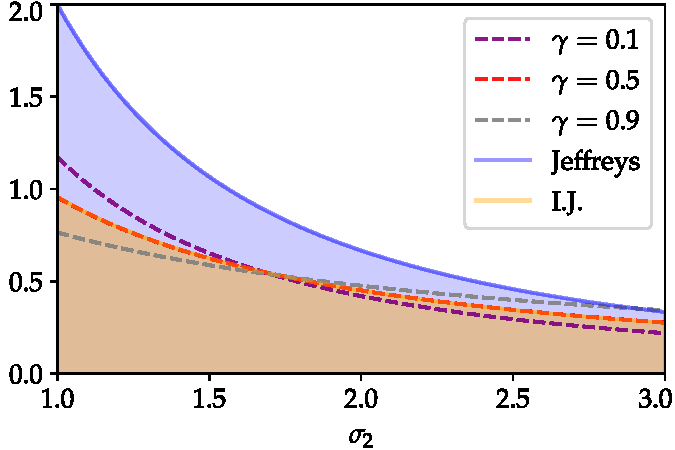
\includegraphics[width=6cm]{figures/constrained-priors/priors_.pdf}\hspace*{1cm}%
    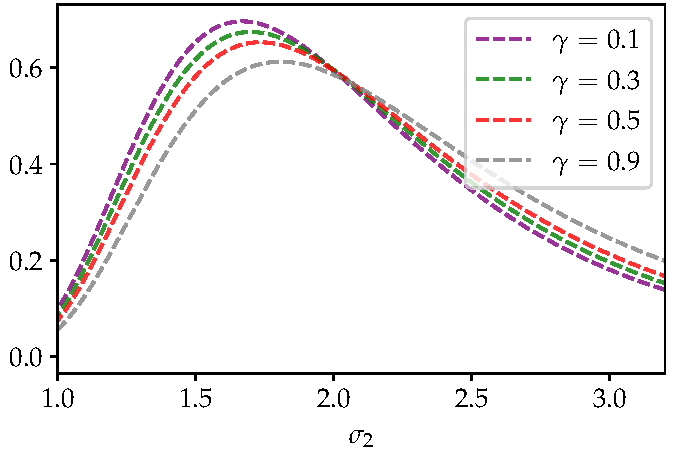
\includegraphics[width=6cm]{figures/constrained-priors/post5.pdf}\\
    \makebox[13cm][c]{%
    {~\hspace{\stretch{1}}(a)\hspace{\stretch{2}}(b)\hspace{\stretch{1}}~}}\\[5pt]
    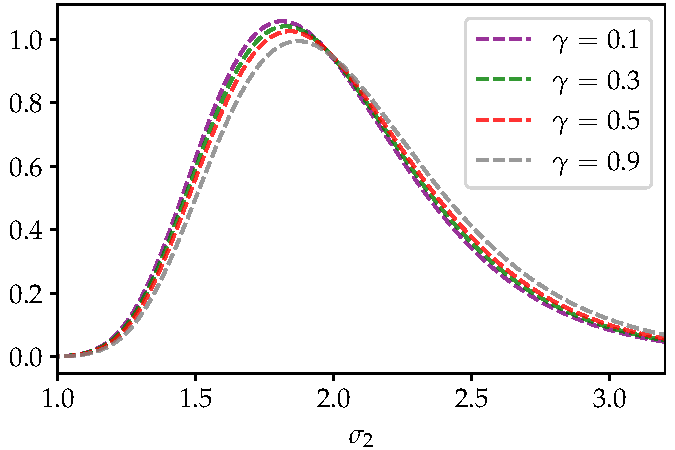
\includegraphics[width=6cm]{figures/constrained-priors/post15.pdf}\hspace*{1cm}%
    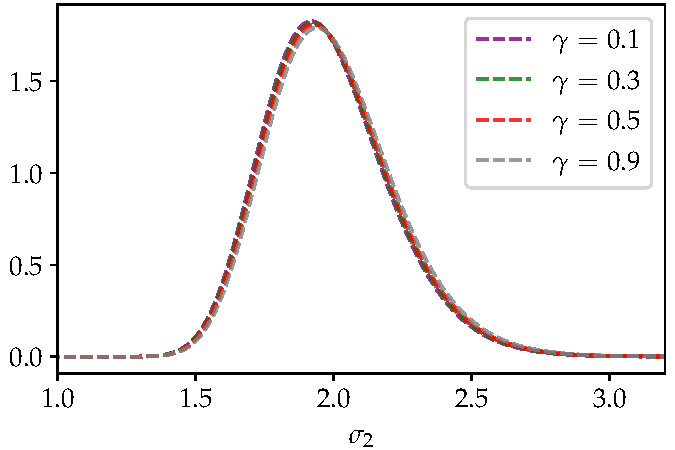
\includegraphics[width=6cm]{figures/constrained-priors/post50.pdf}\\
    \makebox[13cm][c]{%
    {~\hspace{\stretch{1}}(c)\hspace{\stretch{2}}(d)\hspace{\stretch{1}}~}}%
    \caption{On (a), different prior densities $\pi_\gamma$ (in dashed line) w.r.t. $\sigma_2$ along with a Jeffreys prior density (that delimits the blue area) and the \emph{Independent Jeffreys} of \cite{rubio_inference_2014} (that delimits the orange area). On each of (b), (c) and (d), posterior densities for different values of $\gamma$ are plotted. %One observed sample served the calculation of all the posteriors on one figure. 
    One observed sample was used to calculate all the posteriors in a figure.
    The observed sample has a size of $k=5$ in (b), $k=15$ in (c), and $k=50$ in (d).\label{fig:priorpost}}
\end{figure}








\section{Detailed proofs}\label{sec:BA:proofs}


\subsection{Proof of \cref{thm:Jthetaa}}

To prove this theorem, we consider to simplify the derivations that $b=0$ with $\Theta=(0,1]$. We will show later how to extend the result to the other cases. As the Jeffreys prior can be defined up to a positive multiplicative constant with no incidence on the definition of a $D_\delta$-reference prior, 
we will simplify its decay rate assuming $J(\theta)\equi{\theta\rightarrow 0}\theta^a$.

Let us define the increasing sequence of compact subsets $\Theta$: $\Theta_i=[\theta_i,1]$, $i\geq0$, with $\theta_i\conv{i\rightarrow\infty}0$. We denote by $\psi_i$ and $\tilde\psi_i$ the functions defined as follow:
    \begin{equation}
        \psi_i(u) = -\frac{\int_{\Theta_i}J(\theta)^{-\delta}\theta^{u(1+\delta)}d\theta }{\left(\int_{\Theta_i}\theta^ud\theta \right)^{1+\delta}},\qquad \tilde\psi_i(u) = -\frac{\int_{\Theta_i}\theta^{-a\delta }\theta^{u(1+\delta)}d\theta }{\left(\int_{\Theta_i}\theta^ud\theta \right)^{1+\delta}}.
    \end{equation}
The quantity $\psi_i(u)$ corresponds ---up to a positive constant--- to the parametrization w.r.t. $u\in\RR$ of $l(\pi_i)$; where $\pi(\theta)\propto\theta^u$, $\pi_i$ is re-normalized restriction of $\pi$ to $\Theta_i$  and where $l$ is the function defined in \cref{thm:BA:l(pi)} that we seek to maximize.
Therefore, if we call $u_i\in\argmax_{u\in\RR}\psi_i(u)$ for any $i$, and if the associated sequence of priors $(M(\pi_i))_i$ converge Q-vaguely to a prior $\varPi^\ast$ over $\Theta$, that would prove that $\varPi^\ast$ is a quasi $D_\delta$-reference prior.

\paragraph{The case $\mathbf{a<-1}$}
    Firstly, we assume that $a<-1$. Denote $U=(-\infty, u_m:=\frac{\delta a-1}{1+\delta})$, we want to derive an asymptotic equivalent when $i\to\infty$ of $\psi_i(u)$, uniformly w.r.t. $u\in U$.
    More precisely, we are about to show that for any $\eps>0$ there exists a $i_1$ such that for any $u\in U$ and $i>i_i$, $|\psi_i(u)-\tilde\psi_i(u)|<\eps|\tilde\psi_i(u)|$. %\theta_i^{-\delta(a+1)}$.
    

    Let $\eps>0$, using that $J(\theta)^{-\delta}\equi{\theta\rightarrow0}\theta^{-\delta a}$, there exists $i_0$ such that for any $\theta<\theta_{i_0}$, $|J(\theta)^{-\delta}-\theta^{-\delta a}|<\eps\theta^{-\delta a}$. %for a $\tilde\eps$ that we determine later.
    Now, we consider an $i_1$ such that: % for any $u\in U$:
        \begin{equation}
            \frac{\int_{\Theta_{i_0}}J(\theta)^{-\delta}d\theta }{\int_{\theta_{i_1}/\theta_{i_0}}^1J(\theta_{i_0}\theta)^{-\delta}\theta^{u_m(1+\delta)} d\theta}<\theta_{i_0}\eps/2\quad \text{and}\quad
            \frac{\int_{\Theta_{i_0}}\theta^{-\delta a}d\theta }{\int_{\theta_{i_1}/\theta_{i_0}}^1(\theta_{i_0}\theta)^{-\delta a}\theta^{u_m(1+\delta)} d\theta}<\theta_{i_0}\eps/2.
        %
            % \frac{\int_{\Theta_{i_0}} J(\theta)^{-\delta}\theta^{u(1+\delta)}  d\theta}{\int_{\Theta_{i_1}\setminus\Theta_{i_0} } J(\theta)^{-\delta }\theta^{u(1+\delta)}d\theta }
            % = 
            % \frac{\theta_{i_0}^{-1}\int_{\theta_{i_0}}^1 J(\theta)^{-\delta}(\frac{\theta}{\theta_{i_0}})^{u(1+\delta)}  d\theta}{\int_{\theta_{i_1}/\theta_{i_0}}^1 J(\theta_{i_0}\tilde\theta)^{-\delta }\tilde\theta^{u(1+\delta)} d\tilde\theta }
            % %
            % < \frac{\theta_{i_0}^{-1}\int_{\Theta_{i_0} }J(\theta)^{-\delta} d\theta}{\int_{\theta_{i_1}/\theta_{i_0} }^1 J(\theta_{i_0}\theta)^{-\delta }\theta^{u^m(1+\delta)}d\theta}
        \end{equation}
    Thus, for any $i>i_1$  and any $u\in U$:
        \begin{equation}
            \frac{\int_{\Theta_{i_0}} J(\theta)^{-\delta}\theta^{u(1+\delta)}  d\theta}{\int_{\Theta_{i}\setminus\Theta_{i_0} } J(\theta)^{-\delta }\theta^{u(1+\delta)}d\theta }
            = 
            \frac{\theta_{i_0}^{-1}\int_{\theta_{i_0}}^1 J(\theta)^{-\delta}(\frac{\theta}{\theta_{i_0}})^{u(1+\delta)}  d\theta}{\int_{\theta_{i}/\theta_{i_0}}^1 J(\theta_{i_0}\theta)^{-\delta }\theta^{u(1+\delta)} d\theta } %\\
            %
            < \frac{\theta_{i_0}^{-1}\int_{\Theta_{i_0} }J(\theta)^{-\delta} d\theta}{\int_{\theta_{i_1}/\theta_{i_0} }^1 J(\theta_{i_0}\theta)^{-\delta }\theta^{u_m(1+\delta)}d\theta} < \eps/2
        \end{equation}
    and
        \begin{equation}
            \frac{\int_{\Theta_{i_0}} \theta^{-\delta}\theta^{u(1+\delta)}  d\theta}{\int_{\Theta_{i}\setminus\Theta_{i_0} } \theta^{-\delta }\theta^{u(1+\delta)}d\theta }
            = 
            \frac{\theta_{i_0}^{-1}\int_{\theta_{i_0}}^1 \theta^{-\delta}(\frac{\theta}{\theta_{i_0}})^{u(1+\delta)}  d\theta}{\int_{\theta_{i}/\theta_{i_0}}^1 (\theta_{i_0}\theta)^{-\delta }\theta^{u(1+\delta)} d\theta } %\\
            %
            < \frac{\theta_{i_0}^{-1}\int_{\Theta_{i_0} }\theta^{-\delta} d\theta}{\int_{\theta_{i_1}/\theta_{i_0} }^1 (\theta_{i_0}\theta)^{-\delta }\theta^{u_m(1+\delta)}d\theta} < \eps/2,
        \end{equation}
    so that $|\psi_i(u)-\tilde\psi_i(u)|<\tilde\eps|\tilde\psi_i(u)|$ as expected. %Finally, deriving $\tilde\psi_i(u)$ gives
        %\begin{equation}
         %   |\psi_i(u)-\tilde\psi_i(u)|<\tilde\eps  |u+1|^\delta K\theta_i^{-\delta(a+1)}\frac{1-\theta_i^{-(\delta(u-a)+u+1)}}{(1-\theta_i^{-u-1})^{1+\delta}} <\tilde\eps |u+1|^\delta K'\theta_i^{-\delta(a+1)}
        %\end{equation}        
    %for some constants $K,\,K'>0$, using that $\theta_i^{-u-1}\leq\theta_i^{-u_m-1}<1$ and that$\theta_i^{-(\delta(u-a)+u+1)}\leq\theta_i^{-(\delta(u_m-a)+u_m+1)}\leq1$. Hence the expected result when $\tilde\eps=\eps/K$.

    Now we want to use this asymptotic equivalence to bound the difference $|a-u_i|$, where $u_i$ is defined as a maximal argument of $\psi_i$. The next step is thus to show that such $(u_i)_i$ exists.
    
    There exist $\tilde K$, $\tilde K'$ such that $\tilde K\theta^{-\delta}\leq J(\theta)^{-\delta}\leq \tilde K'\theta^{-\delta}$. 
    Let $i\geq0$, we can write
        \begin{equation}\label{eq:gendarmeJeffreys}
            \tilde K |\tilde\psi_i(u)| \leq|\psi_i(u)| \leq \tilde K'|\tilde\psi_i(u)|
        \end{equation}
    with 
        \begin{equation}
            |\tilde\psi_i(u)| = \theta_i^{-\delta(a+1)}\frac{|u+1|^{1+\delta}}{|\delta(u-a)+u+1|}\frac{1-\theta_i^{-\delta(u-a)-u-1}}{(1-\theta_i^{-u-1})^{1+\delta}}  \conv{u\rightarrow-\infty}+\infty.
        \end{equation}
    That makes $|\psi_i|$ being a coercive and continuous function on $U$, so that it admits minimal arguments in $U$. We denote by $u_i$ one of them: 
        \begin{equation}
            u_i \in \argmax_{u\in U} \psi_i(u).
        \end{equation}

    We recall that, by concavity of $x\mapsto -x^{-\delta}$, we find that $a$ is the only maximal argument of $\tilde\psi_i$ for any $i$. 
    This way, for $i>i_1$, we write
        \begin{align}
            |\tilde\psi_i(u_i)-\tilde\psi_i(a)|&\leq |\psi_i(u_i)-\tilde\psi_i(u_i)| +  |\psi_i(a)-\tilde\psi_i(a)| + |\psi_i(u_i)-\psi_i(a)| \nonumber\\
            \tilde\psi_i(a) - \tilde\psi_i(u_i) &%\leq \eps(|u_i+1|^\delta+ |a+1|^\delta) \theta_i^{-\delta (a+1)} + \psi_i(u_i)-\psi_i(a),
            \leq \eps(|\tilde\psi_i(u_i)|+|\tilde\psi_i(a)|)+ \psi_i(u_i)-\psi_i(a),
        \end{align}
    which leads to 
        \begin{align}
            2(\tilde\psi_i(a)-\tilde\psi_i(u_i)) &%\leq  \eps(|u_i+1|^\delta+ |a+1|^\delta) \theta_i^{-\delta (a+1)} + \psi_i(u_i)-\tilde\psi_i(u_i)+\tilde\psi_i(a)-\psi_i(a) \nonumber\\
            \leq \eps(|\tilde\psi_i(u_i)|+|\tilde\psi_i(a)|) +  \psi_i(u_i)-\tilde\psi_i(u_i)+\tilde\psi_i(a)-\psi_i(a) \nonumber\\
            \tilde\psi_i(a) - \tilde\psi_i(u_i) &%\leq \eps (|u_i+1|^\delta+ |a+1|^\delta) \theta_i^{-\delta (a+1)}.
            \leq \eps(|\tilde\psi_i(u_i)|+|\tilde\psi_i(a)|).
        \end{align}
    %The above work allows to conclude that
    %Within the last inequality above, 
    Consequently to the convergence of
     $(\theta_i^{\delta(a+1)}\tilde\psi_i(a))_i$ toward a positive limit when $i\to\infty$, we deduce that $\theta_i^{\delta(a+1)}(\tilde\psi_i(a)-\tilde\psi_i(u_i))/|\theta_i^{\delta(a+1)}\tilde\psi_i(u_i)|$ is asymptotically null. This prevents the sequence $(\theta_i^{\delta(a+1)}\tilde\psi_i(u_i))_i$ to admit a non finite subsequential limit, meaning it has to be bounded and to converges to the same limit as $(\theta_i^{\delta(a+1)}\tilde\psi_i(a))_i$, i.e. $-|a+1|^\delta$.

     On another hand, we notice that for any $M>0$, there exist a $M'$ such that for any $u<M'$, 
        \begin{equation}
            \frac{|u+1|^{1+\delta}}{|\delta(u-a)+u+1|}>M
        \end{equation}
     and $|\theta^{\delta(a+1)}\tilde\psi_i(u)|>M$ for any $i\geq0$. Thus, as $(\theta^{\delta(a+1)}\tilde\psi_i(u_i))_i$ has been proven to be bounded, so must be $(u_i)_i$.

     To conclude on that sequence, we denote by $\rho$ a finite subsequential limit of $(u_i)_i$, if $\rho\ne u_m$ then deriving the limit of $\theta^{\delta(a+1)}\tilde\psi_i(u_i)$ leads to 
        \begin{align}
           & -\frac{|\rho+1|^{1+\delta}}{\delta(\rho-a)+\rho+1} = |a+1|^\delta \nonumber\\
           \text{i.e.}\quad & -|\rho+1|(|\rho+1|^\delta-|a+1|^\delta) = |a+1|^\delta \delta(\rho-a);
        \end{align}
    necessarily, $\rho=a$.
    It remains to prove that $\rho=u_m$ is absurd. Indeed, in this case the integrals $\int_{\Theta_i}\theta^{-\delta a+u_i(1+\delta)}d\theta$ converge either to $0$, either to $+\infty$. Therefore, that would make $(\theta_i^{\delta(a+1)}\tilde\psi_i(u_i))_i$ converging either to $-\infty$, either to $0$, which in both case is different to $-|a+1|^\delta$.


    %Eventually, $(u_i)_i$ converges to $a$.

    Let us now work beyond the subset $U$ of $\RR$. First, if $u\in(-1,+\infty)$, the integrals that compose $\psi_i(u)$ both admit finite and positive limits when $i\to\infty$. The limit of $(|\psi_i(u)|)_i$ is moreover bounded from below as a consequence of \cref{eq:gendarmeJeffreys}:
        \begin{equation}\label{eq:minorationpsiu1infty}
            |\psi_i(u)|\geq \tilde K\frac{(u+1)^{1+\delta}}{ \delta(u-a)+u+1}\frac{1-\theta_i^{\delta(u-a)+u+1}}{(1-\theta_i^{u+1})^{1+\delta}} \geq \tilde K'|\log\theta_i|^{-1-\delta}.  %{(\mu+1)^{\delta}}. %\conv{i\rightarrow\infty}\infty
        \end{equation}
    %and the same way, $\psi_i(-1)\geq\tilde K\frac{(\log\theta_i)^{-1-\delta}}{|\delta(1+a)|}$
    Thus, there exists $i_2\geq0$ such that for any $i>i_2$ $|\psi_i(a)|<\tilde K'|\log\theta_i|^{-1-\delta}$, consequently to $\psi_i(a)\equi{i\rightarrow\infty}|a+1|^{\delta}\theta_i^{-\delta(a+1)}\aseq{i\rightarrow\infty}o(|\log\theta_i|^{-\delta-1})$.
    As a result, for any $i>i_2$:
        \begin{equation}
            \sup_{u\in(-1,+\infty)}\psi_i(u)<\psi_i(a)\leq\psi_i(u_i).
        \end{equation}
    Finally, if $u\in(u_m,-1)$, analogously than in \cref{eq:minorationpsiu1infty}, we can write
        \begin{equation}
            |\psi_i(u)|\geq\tilde K(u+1)^{1+\delta}\frac{|\log\theta_i|}{(1-\theta_i^{u+1})^{1+\delta}} \geq \tilde K''\theta_i^{-(u_m+1)(1+\delta)}|\log\theta_i|^{-\delta}.
        \end{equation}
    Once again, we have $\psi_i(a)\aseq{i\rightarrow\infty}o(\theta_i^{-(u_m+1)(1+\delta)}|\log\theta_i|^{-\delta})$ and we can consider $i_3\geq 0$ such that for any $i>i_3$:
        \begin{equation}
            \sup_{u\in(u_m,-1)}\psi_i(u)<\psi_i(a)\leq\psi_i(u_i).
        \end{equation}

    All the work that precedes proves that any sequence $(v_i)_i$ defined by $v_i\in\argmax_{\RR}\psi_i$ converges to $a$.
    

\paragraph{The case $\mathbf{a=-1}$}
In this case, we easily get that $\psi_i(a)\equi{i\rightarrow\infty}-|\log\theta_i|^{-\delta}$. 
When $u<\eta<a$, 
    \begin{equation}
        |\psi_i(u)|\geq\tilde K\frac{|u+1|^{\delta}}{\delta+1} \frac{1-\theta_i^{-(\delta+1)(u+1)}}{(1-\theta_i^{-u-1})^{1+\delta}}\geq \hat K {|\eta+1|^{\delta}}(1-\theta_i^{-(\eta-1)({1+\delta})})
    \end{equation}
and when $u>\tilde\eta>a$,
    \begin{equation}
        |\psi_i(u)|\geq\tilde K\frac{|u+1|^{\delta}}{\delta+1} \frac{1-\theta_i^{(\delta+1)(u+1)}}{(1-\theta_i^{u+1})^{1+\delta}}\geq \hat K' {|\tilde\eta+1|^{\delta}}(1-\theta_i^{(\tilde\eta-1)({1+\delta})}).
    \end{equation}


Thus, for any $\eps>0$, the equations above with $\eta=a-\eps$ and $\tilde\eta=a+\eps$ let state that there exists an $i_1\geq0$ such that for any $i>i_1$:
    \begin{equation}
        \sup_{u\in(-\infty,a-\eps)}\psi_i(u)<\psi_i(a)\quad\text{and} \quad\sup_{u\in(a+\eps,\infty)}\psi_i(u)<\psi_i(a)
    \end{equation}
so that $\argmax_{\RR}\psi_i\subset(a-\eps,a+\eps)$, which let the definition of a sequence $(u_i)_i$ of maximal arguments of $\psi_i$ which converges to $a$.


\paragraph{Q-vague convergence}
The conclusion concerning the Q-vague convergence of the $M(\pi_i^\ast)$ defined from the $u_i$ constructed in the work above: $\pi_i^\ast(\theta)\propto\theta^{u_i}$ is a direct result of \cite[Proposition 2.16]{bioche_approximation_2016}. Indeed, the convergence of sequence $(u_i)_i$ toward $a$, implies that the sequence of our priors converges Q-vaguely to $\varPi^\ast$ such that $\varPi^\ast = M(\pi^\ast)$ with $\pi^\ast(\theta)\propto{\theta^a}$.



\paragraph{Extension to other set $\Theta$}
We shall now demonstrate that the proven result extends itself to the general case: $\Theta=[c,b)$ or $(b,c]$, $b\in\RR\cup\{-\infty,\infty\}$.

We first consider $\Theta=(b,c]$ with $b\in\RR$.
We denote by $\cQ$ the set of priors densities after the substitution $\vartheta = (\theta-b)/(c-b)\in T=(0,1)$:  $\cQ=\{\tilde\pi(\vartheta) = (b-c)\pi(\vartheta (b-c)+b),\,\pi\in\hat\cR\}$.
Thus, $\cQ = \{\pi(\theta)\propto\vartheta^u,\,u\in\RR\}$.
We define the increasing sequence of compact sets $(\Theta_i)_i$ by $\Theta_i = [b+t_i,c]$ with $t_i\conv{i\rightarrow}0$. Therefore, for $\pi\in\hat\cP$, calling $\pi_i$ the renormalized restriction of $\pi$ to $\Theta_i$ gives
    \begin{equation}
        l(\pi_i) = \tilde l(\tilde\pi_i) = C_\delta\int_{T_i}\tilde\pi_i(\vartheta)^{1+\delta}\tilde J(\vartheta)^{-\delta}d\vartheta
    \end{equation}
with $T_i=[t_i,1]$, $\tilde\pi_i(\vartheta) = (b-c)\pi_i(\vartheta (b-c)+b)\in\cQ$ and $\tilde J(\vartheta) = (b-c)J(\vartheta (b-c)+b)\equi{\vartheta\rightarrow0}\vartheta^a$.
Thus, the work done above states that the family of maximal arguments $\tilde\pi_i^\ast$ of $\tilde l$ over $\cQ_i$  provides a sequence of priors $(M(\tilde\pi_i^\ast))_i$ that converges Q-vaguely toward $M(\tilde\pi^\ast)$ where $\tilde\pi^\ast(\vartheta)\propto\vartheta^a$.
Thus, the associate densities $\pi^\ast_i$ maximize $l$ over $\cP_i$ and issues a sequence of priors $(M(\pi^\ast_i))_i$ that converges Q-vaguely toward $M(\pi^\ast)$ where $\pi^\ast(\theta)\propto|\theta-b|^a$.

To treat the other cases, other substitutions with analogous work permit to conclude:
(i) the substitution $\vartheta=(b-\theta)/(b-c)$
when $\Theta=(c,b)$, $b\in\RR$; (ii) the substitution $\vartheta=1/(|\theta-c|+1)$ when 
$\Theta=[c,\infty)$ or $(-\infty,c]$.








\subsection{Proof of \cref{prop:constraints}}

Let us start by the uniqueness.
%Recall the definition of an openly increasing sequence of compact sets $(\Theta_i)_{i\in\NN}$: there exist $i_0\geq0$ and a sequence $(V_i)_{i\geq i_0}$ of open subsets of $\Theta$  such that for any $i\geq i_0$
%    \begin{equation}
%        \Theta_i\subset V_i\subset \Theta_{i+1}.
%    \end{equation}
%This way, $\bigcup_iV_i=\Theta$ and the compacity of $\Theta$ imposes it to  be a finite union, so that $\Theta_i=\Theta$ for any $i\geq i_1$ for some $i_1\geq0$.\\
%
%
%If $(\Theta_i)_{i\in \NN}$ is an increasing sequence of compact subsets that covers $\Theta$, %%%($i_1<i_2\Longrightarrow\Theta_{i_1}\subset\Theta_{i_2}$, $$), 
%it is stationary, i.e. there exist an $i_0$ such that for any $i>i_0$, $\Theta_i=\Theta$.\\ %%%finite subset $\tilde I\subset I$ such that $\bigcup_{i\in\tilde I}\Theta_i=\Theta$ (or, if $I$ is totally ordored, there exist $i_0$ such that for any $i>i_0$, $\Theta_i=\Theta$).\\
%Indeed, by contradiction assuming that for any $n$, $\bigcup_{i\leq n}\Theta_i\ne\Theta$, its complementary is non-empty and contains a non-empty closed subset $F_n\subset\left(\bigcup_{i\leq n}\Theta_i\right)^c$. Therefore, as $\Theta\subset\RR^d$ it is an Hausdorff compact set so that the two closed sets $F_n$ and $G_n=\bigcup_{i\leq n}\Theta_i$ are subsets of two disjoints open sets $U_n$ and $V_n$: $F_n\subset U_n$, $G_n\subset V_n$. This way, $\bigcup_{n\in\NN}V_n=\Theta$ and by compactness there exists $N$ such that $V_N=\Theta$ and so $F_N=\empty$ which is a contradiction.
%
%Any $D_\delta$-reference prior
A prior $\varPi^\ast\in\cP$ is a $D_\delta$-reference prior if and only if its density $\pi^\ast$ maximizes $l$ over $\cR$, where $M(\cR)=\cP$.
As the set $\cP$ is convex, $\cR$ is convex as well. Also, we notice that the function $\pi\mapsto l(\pi)$ is strictly concave, so that its maximizer is unique in the sense that two maximizer are equal $\nu$-a.e. That ensures the $D_\delta$-reference prior is unique.
%$\pi^\ast$ over a convex   such as $\tilde\cP$ must maximize $l$ as a prior on $\Theta$. The mapping $\pi\mapsto l(\pi)$ being strictly convex when $\pi$ is seen as a function in $\cR^\cC$, such maximal argument is unique.


% Regarding the expression of $\pi^\ast$,it can be seen as a direct consequence of the following lemma, which proven later on.

% \begin{lem}\label{lem:constrainstaec0}
%     Calling $U$ the set of positive and a.e. continuous function from $\Theta$ to $\RR$, and $C=\{f:\Theta\to\RR,\, \int_\Theta f=1,\,\forall j,\,\int_\Theta f_jg_j=c_j\}$, if $\pi^\ast=\argmax_{\pi\in C\cap U}l(\pi)$ exists, it verifies
%         \begin{equation}\label{eq:lemconstepiast}
%             \pi^\ast(\theta)  J(\theta)\left(\lambda_0+\sum_{j=1}^p\lambda_jg_j(\theta)\right)^{1/\delta},
%         \end{equation}
%     for some $\lambda_j\in\RR$. Reciprocally, if there exists a $\pi^\ast\in C\cap U$ that satisfies above equation for some $\lambda_j\in\RR$, then it maximizes $l$ over $C\cap U$.
% \end{lem}




% \paragraph{Proof of Lemma {lem:constrainstaec0}}
Regarding the expression of $\pi^\ast$,
let us call $E$ the space of bounded a.e. continuous functions from $\Theta$ to $\RR$ and we equip $E$ with the supremum norm over $E$: $\|f\|=\sup_\Theta|f|$. The set $\Theta$ being supposed compact, the pair $(E,\|\cdot\|)$ constitutes a Banach vector space whose restriction $U$ composed by the positive functions of $E$ is an open and convex subset.
It is possible to see $l$ as being a concave function defined on $U$.


Let us compute the differentiate of $l$ over $U$. One can write $l=\phi_2\circ\phi_1$ with
\begin{equation}
    \phi_1:\pi\in E\longmapsto \pi^{1+\delta}\in E ;\qquad \phi_2:\pi\in E\longmapsto C_\delta \int_\Theta \pi(\theta)|\cI(\theta)|^{-\delta/2}d\theta.
\end{equation}
As $\phi_2$ is a continuous linear mapping from $E$ to $\RR$, $l$ is differentiate while $\phi_1$ is, with for any $h\in E$:
    \begin{equation}
        dl(\pi) = \phi_2\circ d\phi_1(\pi).
    \end{equation}
Fix $\pi\in U$. For an $\eps>0$ there exists $\tilde\eps>0$ such that while $|x|<\|\pi\|$ and $|u|<\tilde\eps$ then $|(x+u)^{1+\delta}-x^\delta-(1+\delta)x^\delta u|<\eps|u|$. Thus for any $h\in E$ such that $\|h\|<\tilde\eps$, we have
    \begin{equation}
        \|\phi_1(\pi+h) -\phi_1(\pi)-(1+\delta)\pi^\delta h\|<\eps\|h\|.
    \end{equation}
We conclude that $\phi_1$ differentiable on $U$ with $d\phi_1(\pi)h = (1+\delta)\pi^\delta h$, for any $\pi\in U$, $h\in E$. This differentiate is additionally continuous, which makes $l$ continuously differentiable as well.

Thus, considering the additional constraint $\int_\Theta\pi(\theta)d\theta=1$, this problem can be treated applying the Lagrange multipliers theorem (see e.g. \citep{zeidler_applied_2012}) to state that there exist $\lambda_0,\dots,\lambda_p\in\RR^{p+1}$ such that
    \begin{equation}
        dl(\pi^\ast)h - \lambda\int_\Theta h(\theta)d\theta - \sum_{i=1}^p\lambda_i\int_\Theta h(\theta)g_i(\theta)d\theta = 0
    \end{equation}
for any $h\in E$. Eventually, as $dl(\pi)h=C_\delta(1+\delta)\int_\Theta\pi(\theta)^{\delta}|\cI(\theta)|^{-\delta/2}h(\theta)d\theta$, we get
    \begin{align}
        \pi^\ast(\theta) = J(\theta)\bigg(\lambda_0+\sum_{i=1}^p\lambda_ig_i(\theta)\bigg)^{1/\delta}.
    \end{align}
% with $J(\theta$

Moreover,
as $l$ is strictly concave and the constraints are linear, the second order condition for the Lagrangian states the reciprocal aspect of this result: calling $C$ the space of functions satisfying the constraints, if $\pi^\ast\in U\cap C$ satisfies the last equation above, it maximizes $l$.


%To conclude, notice that densities of non-negative priors satisfying the constraints constitute %belongs to 
%the closure of $U\cap C$, $C$ designing the set of the functions that satisfy the constraints. As $\pi^\ast$ disclosed above maximizes $l$ over $U\cap C$, with $l$ being continuous on its closure. Therefore, $\pi^\ast$ maximizes $l$ over all that latter, i.e. its associated prior is the $D_\delta$-reference prior over $\tilde\cP$.

To conclude, the elements in $\tilde\cP$ are associated to densities which belong to $E$ because $\Theta$ is compact.
They are non necessarily everywhere positive, but only supposed to be non-negative.
This set of bounded a.e. continuous and non-negative functions satisfying the constraints is actually the closure of $U\cap C$ over which $l$ is continuous.
Therefore, calling $\tilde\cP^\ast$ the set of positive priors in $\tilde\cP$, we have $\argmax_{M(\pi)\in\tilde\cP}l(\pi)=\argmax_{M(\pi)\in\tilde\cP^\ast}l(\pi)$ which is $\pi^\ast$.








\subsection{Proof of \cref{thm:lintoproper}}


Assuming that it exists, denote by $\pi^\ast$ the density of the $D_\delta$-reference prior $\varPi^\ast$ over $\overline\cP$, denote as well
    \begin{equation}
        c = \int_{\Theta}\pi^\ast(\theta)g(\theta)d\theta,\quad Z_i = \int_{\Theta_i}\pi^\ast(\theta)d\theta
    \end{equation}
for any $i\in \NN$, considering an openly increasing sequence $(\Theta_i)_{i\in\NN}$ of compact sets that cover $\Theta$ over which $1>\varPi^\ast(\Theta_i)>0$ for any $i$ such that $\Theta_i\ne\Theta$ (we show later that they exist).
In particular, $\varPi^\ast$ must be the $D_\delta$-reference prior over the set $\cP^c=\{\varPi\in\sM_{\cC}^\nu,\,\int_\Theta gd\varPi =c\}$. %\subset\cP$.

Let $i\in \NN$, if $\pi_i$ is a density on $\Theta_i$ such that 
\begin{equation}
    \int_{\Theta_i}\pi_ig + \frac{1}{Z_i}\int_{\Theta\setminus\Theta_i}\pi^\ast g = \frac{c}{Z_i},
\end{equation}
then the prior whose density $\pi$ on $\Theta$ defined by $\pi=Z_i\pi_i+\pi^\ast\indic_{\Theta\setminus\Theta_i}$ %as being proportional to $\pi_i$ on $\Theta_i$ and on $\pi^\ast$ on $\Theta\setminus\Theta_i$ 
belongs to $\cP^c$.
Therefore, denoting $\pi^\ast_i$, the renormalized restriction of $\pi^\ast$ to $\Theta_i$, $l(\pi^\ast_i)$ must be larger than $l(\pi_i)$ on $\Theta_i$ by definition of the reference prior.

Thus, $\pi^\ast_i$ is a maximal argument of $l$ under the constraints 
    \begin{equation}
        \int_{\Theta_i}\pi_i = 1,\qquad \int_{\Theta_i}\pi_i g=\frac{c}{Z_i}-\frac{1}{Z_i}\int_{\Theta\setminus\Theta_i}\pi^\ast g.
    \end{equation}
Given the result of \cref{prop:constraints}, $\pi^\ast_i$ takes the form of:
    \begin{equation}
        \pi^\ast_i = J\cdot(\lambda^{(1)}_i+\lambda^{(2)}_ig)^{1/\delta}
    \end{equation}
for some $\lambda_i^{(1)}$ and $\lambda_i^{(2)}$.

Then, denoting as well $\pi^\ast_{i+1}=J\cdot(\lambda^{(1)}_{i+1}+\lambda^{(2)}_{i+1}g)^{1/\delta}$, and reminding that $\pi^\ast_{i+1}\propto\pi^\ast_i$ on $\Theta_i$, we deduce that $\lambda^{(1)}_{i+1}=\lambda^{(1)}_{i}$ as well as $\lambda^{(2)}_{i+1}=\lambda^{(2)}_{i}$.
Eventually, $\pi^\ast\propto J\cdot (\lambda_1+\lambda_2g)^{1/\delta}$.
Thus, in the neighborhood of $b$, $\pi^\ast(\theta)\equi{\theta\rightarrow b}K\lambda_1^{1/\delta}$ for some $K\ne0$ if $\lambda_1$ is non-null, which is discordant with the satisfaction of the constraint $\int_\Theta\pi^\ast g<\infty$ in the case where $\int_\Theta Jg=\infty$ or with the constraint $\int_\Theta\pi^\ast =1$ otherwise.


Finally, $\pi^\ast$ is proportional to $Jg^{1/\delta}$ and the value of $c$ must be fixed by
\begin{equation}
    c = \left(\int_\Theta J\cdot g^{1+1/\delta}\right)\cdot\left(\int_\Theta J\cdot g^{1/\delta}\right)^{-1}.
\end{equation}

To finish the proof, we still have to show that $\varPi^\ast$ is not null on any of the $\Theta_i$, or on any of the $\Theta\setminus\Theta_i$. First, there must exist $i_0$ such that $\varPi^\ast(\Theta_{i_0})>0$, so that $\varPi^\ast(\Theta_i)>0$ for any $i\geq i_0$ and the sequence $(\Theta_i)_{i\geq i_0}$ can be considered instead of the initial one. Second, for any $i$, if $\Theta\setminus\Theta_i$ is non-empty then it has a non-empty interior, as a consequence of the definition of openly increasing sequences of compact sets. Thus, as $\varPi^\ast$ is assumed to be positive, $\varPi^\ast(\Theta\setminus\Theta_i)$ is non-null. Hence the result.



\subsection{Proof of \cref{thm:quasipostpropre}}

  Consider an openly increasing sequence of compact sets $(\Theta_i)_{i\in\NN}$ that covers $\Theta$. Let $i\in\NN$, for $\varPi$ to be a $D_\delta$-reference prior over $\cP_i$, its normalized density $\pi_i$ %---associated to its probability density on $\Theta_i$--- 
  %to be a reference prior over $\cP_i$, it 
  must maximize the function $l$ under the constraints $\int_{\Theta_i}\pi_i=1$ and $\int_{\Theta_i}\pi_i g=c_i$. Thus, according to \cref{prop:constraints}, $\pi_i$ can be written as:
     \begin{equation}
         \pi_i(\theta)\propto J(\theta)(\lambda_i^{(1)}+\lambda_i^{(2)}g(\theta))^{1/\delta},
     \end{equation}
 for some $\lambda_i^{(1)}$ and $\lambda_i^{(2)}$.
 Considering, if required, a subsequence of $(\pi_i)_{i\in\NN}$, we can assume that $\lambda_i^{(1)}$ and $\lambda_i^{(2)}$ have constant signs.
 Also, by convexity we write:%
 \newcommand{\li}[1]{\lambda_i^{(#1)}}%
     \begin{align}\label{eq:convexityConsCpig}
         c_i^\delta  & \geq \int_{\Theta_i}J(\theta)(\li1+\li2g(\theta))g(\theta)d\theta\left(\int_{\Theta_i}Jg\right)^{\delta-1}  \\
         &\geq \li1\left(\int_{\Theta_i}Jg\right)^{\delta} + \li2\frac{\int_{\Theta_i}Jg^{2} }{\left(\int_{\Theta_i}Jg\right)^{1-\delta}},\nonumber
     \end{align}
    and
    \begin{align}\label{eq:convexityConspi1}
        1 & \geq \int_{\Theta_i}J(\theta)(\li1+\li2g(\theta))d\theta\left(\int_{\Theta_i}J\right)^{\delta-1} \\
        &\geq \li1\left(\int_{\Theta_i}J\right)^\delta + \li2 \frac{\int_{\Theta_i}Jg}{\left(\int_{\Theta_i}J\right)^{1-\delta}}  . \nonumber
    \end{align}
We want to identify the possible subsequential limits of $\li1$. 
We assume that one exists in $(0,\infty]$, we can consider if required a subsequence to assume that it is the actual the limit of $\li1$. 
This way, \cref{eq:convexityConspi1} does not allow $\li2$ to be non-negative.
Thus, $\li2$ is negative and by convexity,
 %  \begin{equation}
 %       1\geq \li1\left(\int_{\Theta_i}J\right)^\delta + \li2\frac{\left(\int_{\Theta_i} Jg^{1+1/\delta}\right)^{\delta/(1+\delta)}}{\left(\int_{\Theta_i}J\right)^{1-\delta}} \left(\int_{\Theta_i}J\right)^{1/(1+\delta)}
 %   \end{equation}
 %   or
    \begin{equation}\label{eq:convixity2l2leq0}
        c_i^\delta \geq \li1\left(\int_{\Theta_i} Jg\right)^\delta +\li2 \left(\int_{\Theta_i} Jg^{1+1/\delta}\right)^\delta .
    \end{equation}
%
  %  $$\frac{1}{1+\delta}-1+\delta = \frac{\delta^2}{1+\delta}\in(0,\delta)\qquad$$
 Given that $(c_i)_i$ is bounded, and that $\int_{\Theta_i}Jg\conv{i\rightarrow\infty}\infty$ while $\int_{\Theta_i}Jg^{1+1/\delta}$ has a finite limit, we deduce that $\li2$ diverges to $-\infty$.
 However, to ensure the expression of $\pi_i$ to be well defined, we must have $\li1+\li2g(\theta)\geq0$ for any $i$ and any $\theta$. As $g$ is non-null, it necessary comes that $(\li2/\li1)_i$ is a  bounded sequence.
Therefore, 
%\begin{equation}
%    \li2 \aseq{i\rightarrow\infty} o\left(\li1\left(\int_{\Theta_i}Jg\right)^\delta\right)    
%\end{equation}
$\li2 \aseq{i\rightarrow\infty} o\left(\li1\left(\int_{\Theta_i}Jg\right)^\delta\right) $
and the right hand side in \cref{eq:convixity2l2leq0} diverges to $\infty$, which is a contradiction with $(c_i)_i$ being bounded.

As a consequence, any subsequential limit of $(\li1)_i$ must belong to $[-\infty,0]$. Without changing the notations, we can now assume that $(\li1)_i$ has a limit, which we suppose to be strictly negative firstly, also, $(\li1)_i$ can then be assumed to be always negative.
 Thus, still to ensure that $\li1+\li2g(\theta)\geq0$ for any $i$, $\theta$, and reminding that $g(\theta)\conv{\theta\rightarrow b}0$ we deduce $\frac{\li2}{|\li1|}\conv{i\rightarrow\infty}\infty$.
 Then, 
 the sequence of functions $\left(\pi_i/\li2\right)_i$ converges pointwisely to $\pi^\ast$, defined by $\pi^\ast(\theta)\propto J(\theta)g(\theta)^{1/\delta}$ with  $|\frac{1}{\li2}\pi_i(\theta)|\leq C+g(\theta)$ for some $C$, with $g$ being bounded on all compact sets. %\footnote{If $g$ is not continuous but belongs to $\cR^\cC$, it is bounded on every compact. Then, \cite[Proposition 2.16]{Bioche2016} allows to conclude.}.
According to \cite[Proposition 2.15]{bioche_approximation_2016}, what precedes implies that the sequence of priors $(M(\pi_i))_i$ converges Q-vaguely to $M(\pi^\ast)$.

Eventually, if $(\li1)_i$ admits $0$ as a subsequential limit, 
we can assume that it is its actual limit.
Consequently,  the sequence of functions $(\pi_i/\li2)_i$ converges pointwisely to the density $\pi^\ast$ while being bounded  by $g$. Therefore, the sequence of priors $(M(\pi_i))_i$ converges Q-vaguely to $M(\pi^\ast)$.
%
In any cases, $M(\pi^\ast)$ is a quasi-reference prior over $\overline\cP'$.

 
 
 
 











\section{Conclusion}\label{sec:BA:conclusion}



Prior elicitation remains an open topic in Bayesian analysis, with no solution satisfying all criteria (objectivity, computational feasibility, property, ...) simultaneously. 
In this work, we have focused on the objectivity and exploitability of priors.
Specifically, we have provided some solutions for practitioners seeking non-subjective priors, addressing the practical challenges of traditional reference priors, particularly in terms of complexity and proper aspect. Through the example we presented, we demonstrated that simple criteria can lead to the construction of reference priors that are either straightforward to formulate or proper, depending on the case.

Moreover, our results show that one cannot completely dispense with a consideration of the asymptotic properties of Jeffreys prior. This emphasizes the importance of studying this prior for a complete construction of objective priors.
Indeed, although one of our results  offers a way to define in a simpler way the reference prior when it has improper decay rates, Jeffreys' rate still have to be elucidated. Our other result requires to derive the whole Jeffreys prior.

The approximation of the latter thus becomes a problem of a prior importance. Of course, one can thoroughly focus its explicit expression, yet it can be cumbersome to derive. In the \cref{chap:varp} we propose a numerical solution for the approximation of the Jeffreys prior.

















\chapter{Variational approximation of the reference priors}




\part{Seismic fragility curve estimation}


\chapter{Seismic fragility curves in probabilistic risk assessment studies}



\begin{abstract}
    abstract
\end{abstract}

\minitoc


\section{Introduction}

% The SPRA contains several tools and things

The Seismic Probabilistic Risk Assessment (SPRA) defines a framework and a methodology for the study of seismic structural reliability. %This framework is parrt of the probabilistic 
% As for the Pr
It has been introduced since 1969 \citep{cornell_engineering_1968}
to incorporate the seismic risk evaluation in the probabilistic risk assessment studies.
% and further developed in the
The SPRA has been mostly developed and carried out in the 1980s on nuclear facilities (see e.g. \cite{kennedy_probabilistic_1980,kennedy_seismic_1984}). 
It includes: the determination of the seismic hazard, the analysis of the seismic fragility of structural components, the evaluation of the risks combination and their consequences in the system, as described in the report of the Electric Power Research Institute \citep{epri_seismic_2013}, which provides guidelines for its implementation. %among other ingredients.
%The guidelines for its implementation are thoroughly described in the 
It is since widely used in the nuclear industry (e.g. \cite{ellingwood_validation_1990,park_survey_1998,kennedy_risk_1999}) and its consideration is established among the safety standards adopted by the International Atomic Energy Agency \citep{iaea_probabilistic_2020}.

% Estimating th

Within the SPRA, seismic fragility curves represent a key asset that play a prominent role in the analysis of structural components' fragility step (see  \cite{epri_advanced_2011}).
They express in probabilistic terms the fragility of structures under seismic excitation. We can mention that they are also a tool of interest of performance-based earthquake engineering (PBEE; \cite{ghobarah_performance-based_2001,noh_development_2014}), 
which aims at relating performance objectives to level of damage to the structure.
In any case, they are defined as a function of the seismic hazard, which ---driven by the magnitude (M), the source-site distance (R), and other earthquake parameters--- is reduced to a scalar value derived from the seismic signal: the intensity measure (IM), under the so-called ``sufficiency assumption'' \citep{cornell_hazard_2004,luco_structure-specific_2007}.
In practice, a fragility curve, denoted $P_f$, therefore express the probability of failure of a mechanical structure as a function of an IM value of interest such as peak ground acceleration (PGA) or pseudo-spectral acceleration (PSA), among others:
    \begin{equation}
        P_f(a) = \PP(\text{``failure''}|\text{IM}=a).
    \end{equation}
Within the SPRA framework, the fragility curve expression is expected to be combined with the seismic hazard frequency to compute the damage frequency of the component $C_f$:
    \begin{equation}
        C_f =  \int_0^\infty P_f(a)dH(a).
    \end{equation}
If $H$ is the mean annual  distribution of the IM, $C_f$ represents the annual damage frequency of the component.
It should be noted that the sufficiency assumption was introduced to reduce estimation costs since it assumes that the fragility curve of a given structure is identical regardless of the seismic scenario.
Actually, this assumption embeds some uncertainty in the problem since, as shown in \citeauthor{radu_earthquake-source-based_2018}, \citeyearlink{radu_earthquake-source-based_2018,grigoriu_are_2021}, %\cite{radu_earthquake-source-based_2018,grigoriu_are_2021}, 
different seismic scenarios can lead to identical distributions of some IMs, despite having significantly different frequency contents.
The uncertainty rooted in the fragility curve by this assertion can be classified as an \emph{aleatoric} (irreducible) kind of uncertainty
 (we refer to the \cref{chap:intro-english} for the definition of the uncertainty quantification framework).
% belong to the category of
%The evaluation of the fragility curve defined in eq?? implies the consideration of this
% Focusing the definition of the fragility curve <


In this second part of the manuscript, we focus on the estimation of seismic fragility curves. 
Thus, we do not question the determination of the seismic hazard distribution $H$, nor the derivation of the damage frequency of the component $C_f$.
Nevertheless, estimating the fragility curve itself %for given mechanical equipment 
remains a daunting task. It is commonly done statistically, using different kind of methods depending 
on the source of data available, their characteristics, and their quantity.
This chapter proposes a review of these methods. 
In the next section,
we define the different kind of data involved in the seismic fragility curve estimation in the literature. In particular, we present a stochastic seismic signal generator, and  we present how the failure of mechanical equipment is generally defined.
In section ?? and section ?? different modeling of the fragility curves for its statistical estimation are presented, they are grouped in two categories: non-parametric and parametric.
Explicit examples of case studies are given in section ??, from a theoretical one to an experimental one for which really few data are available.
Given those and the non-exhaustive list of modeling we present from the literature, we question 





% steps of seismic hzarad determination or r
% The derivation 




% it embedds uncertainty suinc...

% that in the step
%As shown in \cite{Radu2018,Grigoriu2021}, different seismic scenarios can however lead to identical distributions of some IMs, although the underlying seismic signals have significantly different frequency contents. As a result, the sufficiency assumption is not met, especially for non-linear, multimodal structures, etc., with current IMs. 
%
%
% Despite this, it is possible to focus on the definition of the resulting fragility curve, without taking the assumption for granted, which is the case in this work.

% and is widely used in in the nuclear industry







% Seismic fragility curves represent a key one. They were introduced in the 1980s for seismic risk assessment studies carried out on nuclear facilities \citep{kennedy_probabilistic_1980,kennedy_seismic_1984,ellingwood_validation_1990,park_survey_1998,kennedy_risk_1999,cornell_hazard_2004}.


% %IN the SPRA, historic, lot of things are defined,
% %among them, the seismic fragility curves. 
% %They represent an essential tool..
% Also used in PBEE, link with insurance?

% IM, sufficientcy assumption. Different, various scenario and methods
% Quantification of uncertainty?


% This chapter suggests a review of the main methods that exist in the literature 




\section{Data: from seismic signals to equipments failures}





In the literature, different source of data are exploited to estimate seismic fragility curves. 
We can cite, for instance:
(i) expert assessments supported by test data (e.g. \cite{kennedy_probabilistic_1980,kennedy_seismic_1984,zentner_fragility_2017}), (ii) experimental data (e.g. \cite{park_survey_1998}), (iii) empirical data from past earthquakes (e.g. \cite{shinozuka_statistical_2000,straub_improved_2008,lallemant_statistical_2015,buratti_empirical_2017,laguerre_empirical_2024}), and (iv) analytical results obtained from various numerical models using artificial or natural seismic excitations (e.g. \cite{ellingwood_earthquake_2001,kim_development_2004,zentner_numerical_2010,koutsourelakis_assessing_2010,mai_seismic_2017,trevlopoulos_parametric_2019,wang_influence_2020,mandal_seismic_2016,wang_seismic_2018,wang_bayesian_2018,zhao_seismic_2020,katayama_bayesian-estimation-based_2021,gauchy_importance_2021,khansefid_fragility_2023,lee_efficient_2023}).
In every of these studies, each sample in 
the dataset regroups:
\begin{enumerate}
    \item Information about a seismic ground motion. The considered ground motions are sometimes natural and sometimes artificial. The information can take several forms, %(such as the temporal signal), 
    as stated in the introduction it is generally used  to derive one or several scalars called intensity measures (IMs).
    % as stated in the introduction, it is generally used to 
    \item Information about the response of the structure or the equipment of interest to the seismic excitation. To define the fragility curve, this information, must permit to characterize the failure of the studied system.
\end{enumerate}
%(i) information about the seismic ground motion (it can be the temporal signal itself,)

In the subsection ?? we pre



Since available records of real seismic excitations for a given site are often scarce, it is common to construct a dataset of artificial earthquake accelerograms using a seismic signal generator.
Various techniques exist for this purpose. According to \citet{rezaeian_stochastic_2008}, the methods can be categorized among the ``source-based'' ones, which model the occurrence of
earthquake rupture at some sources and the propagation of seismic waves to the studied site, and the ``site-based'' ones, which model the seismic signals for the site of interest from the consideration its characteristics and historical recorded earthquake.
A review of the first kind is proposed in \cite{zerva_seismic_1988}, and a review of the second can be found in \cite{shinozuka_stochastic_1988}.
As more recent examples for the latter, we can also cite \cite{trevlopoulos_parametric_2019}; and \cite{zentner_enrichment_2012}.
In the following, we present a stochastic seismic signal generator that is proposed by \citet{rezaeian_simulation_2010}. It lies among the site-based model, and has been implemented by \citet{sainct_efficient_2020}, who calibrated it using $97$ real accelerograms selected in the European Strong Motion Database  for a magnitude $M$ such that $5.5 \leq M \leq 6.5$, and a source-to-site distance $R < 20$~km \citep{ambraseys_dissemination_2000}. 



As said in the introduction, this thesis does not seek to question thoroughly the seismic hazard, and we aim at providing methods that can be applied to any modeling of the seismic signals. Nevertheless, in the following chapters, our methods are applied and validated on different case studies that are presented later on. These case studies take the form of mechanical equipment that have been submitted to artificial seismic signals generated using the generator implemented by \citet{sainct_efficient_2020}, and presented below.


%the case studies that we present and onto which we will apply our methods are excited using



\subsubsection{Seismic signals generator and IMs}

The seismic excitation generated takes the form of a temporal signal that is the realization $s:t\in[0,T]\mapsto s(t)\in\RR$ of a random process $S$ defined on a probability space $(\Omega,\Xi,\PP)$. The generator presented here corresponds to a modulated filtered stochastic white noise with time dependent parameters:
    \begin{equation}
        s(t)= s(t;w,\boldsymbol{\rho},\boldsymbol{\lambda}) = q(t,\boldsymbol\rho)\left[\frac{1}{\sigma_f(t)}\int_{-\infty}^t h(t-\tau,\boldsymbol\lambda(\tau))W(\tau)d\tau \right],
    \end{equation}
where $w$ being a realization of a white noise process $W$. In other terms $W:[0,T]\times\Omega\to\RR$ is such that for all $t_1\ne t_2$, $\EE W(t_1)=0$, $\EE W(t_1)^2=\EE W(t_2)^2$, and $\EE W(t_1)W(t_2)=0$.

The integral in the above equation corresponds to the filtering of $w$, $h(t,\boldsymbol{\lambda})$ being to the impulse response function (IRF) of the linear filter and $\sigma_f$ being its variance: $\sigma_f(t)=\int_{-\infty}^th^2(t-\tau,\boldsymbol{\lambda}(\tau))d\tau$. The IRF is defined by
    \begin{equation}
        h(t-\tau,\boldsymbol{\lambda}(\tau)) = \frac{\omega_f(\tau)}{\sqrt{1-\zeta^2_f}}\exp[-\zeta_f\omega_f(\tau)(t-\tau)]\sin\left(\omega_f(\tau)\sqrt{1-\zeta^2_f}(1-\tau)\right)\indic_{t\geq\tau},
    \end{equation}
where $\boldsymbol{\lambda}(\tau)=(\omega_f(\tau),\zeta_f) $ with $\omega_f(\tau):=\omega_0+\frac{\tau}{T}(\omega_n-\omega)$ being the natural frequency and $\zeta_f\in[0,1]$ being a constant damping ratio. The quantities $\omega_0$ and $\omega_n$ are parameters of the IRF.

 The function $q(t,\boldsymbol\rho)$ is the non-negative modulating function, it is defined by
    \begin{equation}
        q(t,\boldsymbol\rho) = \left\lbrace \begin{array}{ll}
            \rho_1t^2/T_1^2 & \text{if\ } 0\leq t< T_1 \\
            \rho_1 & \text{if\ }T_1\leq t< T_2\\
            \rho_1\exp\left[-\rho_2(t-T_2)^{\rho_3}\right] &\text{if\ }T_2\leq t
        \end{array}\right.
    \end{equation}
where $\boldsymbol\rho=(\rho_1,\rho_2,\rho_3,T_1,T_2)\in(0,\infty)^5$.
Therefore, the signal $s$ depends on $w$ and 
$\boldsymbol{\phi}:=(\boldsymbol{\rho},\omega_0,\omega_n,\zeta_f)\in\boldsymbol{\Phi}:=(0,\infty)^7\times[0,1]$.
The generator consists in deriving realization of $s(\cdot;W,\boldsymbol\phi)$ where 
$\boldsymbol{\phi}$
is stochastic,
its distribution being identified using real acceleration records.
As previously announced,
the records considered are $N_r=97$ real acceleration records form the European Strong Motion Database for a magnitude $M$ such that $5.5\leq M\leq 6.5$ and a source-to-site distance $R<20$~km.
Each of the records corresponds to a realization of $s(\cdot;W,\overline{\boldsymbol{\phi}}_i)$ using a tuple $\overline{\boldsymbol\phi}_i$ as parameters. The distribution of $\boldsymbol{\phi}$ is given by the Gaussian kernel density estimation (see \cite{kristan_multivariate_2011}) of the one of the $(\overline{\boldsymbol\phi}_i)_i$, i.e. its density $p_{\boldsymbol{\phi}}$ is given by
    \begin{equation}
        p_{\boldsymbol{\phi}}(x) \propto \sum_{i=1}^{N_r}\exp\left( -\frac{1}{2} (x-\overline{\boldsymbol\phi}_i)^\top\Sigma^{-1}(x-\overline{\boldsymbol\phi}_i) \right)\indic_{x\in\boldsymbol{\Phi}},
    \end{equation}
where $\Sigma$ is derived from the $(\overline{\boldsymbol{\phi}}_i)_i$ (see \cite{kristan_multivariate_2011}).


From a seismic signal $s$ that is a realization of the process described above, different intensity measure (IM) indicators can be derived.
The choice of the appropriate IM to estimate seismic fragility curves
remains a complex question. 
According to \citet{giovenale_comparing_2004}, the appropriateness of an IM must be defined in terms of efficiency, sufficiency, and hazard compatibility.
However, the most efficient or sufficient IM is not the same for two different case studies (see \cite{mackie_probabilistic_2001,hariri-ardebili_probabilistic_2016}). % changes when a different case 
%regarding the studied system, the results given
% study is considered (see ). 
Moreover, while we do not  thoroughly research the best IM in this thesis, we will see in the following chapters that the best choice is not necessarily simply the one that is the most correlated with the structure's response.
Below we propose a non-exhaustive list of common IMs, a more complete one can be found in \cite{luco_structure-specific_2007}:
    \begin{itemize}
        \item the peak ground acceleration (PGA) is defined as $\text{PGA}=\max_{t\in[0,T]}|s(t)|$;
        \item the peak ground velocity (PGV) is defined as $\text{PGV}=\max_{t\in[0,T]}\left|\int_0^ts(\tau)d\tau \right|$;
        \item the peak ground displacement (PGD) is defined as $\text{PGD}=\max_{t\in[0,T]}\left|\int_{0}^{t}\int_{0}^{\tau}s(u)dud\tau\right|$;
        \item the pseudo spectral acceleration (PSA) at frequency $f_L$ and damping ratio $\xi$ is defined as $\text{PSA}=(2\pi f_L)^2\max_{t\in[0,T]}|x(t)|$, where $x$ is the solution of the linear equation
        \begin{equation}\label{eq:intro-frag:ALS}
            x''(t) + 2\xi2\pi f_Lx'(t)+(2\pi f_L)^2x(t) = -s(t).
        \end{equation}
        This IM is component-dependent since, in practice, the damping ratio $\xi$ and the frequency $f_L$ are evaluated from the mechanical characteristic of the studied system. Generally, the frequency $f_L$ considered for deriving the PSA corresponds to the first mode of the structure's displacement under excitation. \Cref{eq:intro-frag:ALS} corresponds to the displacement equation of the linear single degree of freedom system associated to the structure.
    \end{itemize}





%different IMs


% Regarding seismic ground motions, a common methodology



% SAinct et al

% definition of IMs


\subsubsection{Engineering demand parameter and failure}


As evoked in the preamble of this section, numerous data sources exist for identifying the fragility (and the failure) of mechanical structures and components.





\section{Non-parametric modeling}

MC method,

MC method with 

SVM? GP et  other metamodel?




\section{Parametric modeling}

probit lognormal





\section{Example of case studies}

    \subsection{An elasto-plastic oscillator}

s

    
    \subsection{A piping system from a pressurized water reactor}


s


    \subsection{Stacked structure for storage of packages: typical low data example}

s
    % \subsection{Appropriate modeling with how many data and what data}


\section{Which case study and which data for a Bayesian estimation of fragility curves?}

s


\section{Conclusion}


conclusion





\chapter{Bayesian estimation of seismic fragility: irregular regularization}




\chapter{Design of experiments in a Bayesian framework}


\chapter{Integration of a properly constrained reference prior}




\part{Conclusion \& perspectives}


\appendix
\part*{Appendix}
\addcontentsline{toc}{part}{Appendix}

%\renewcommand{\thechapter}{\Alph{chapter}}

\chapter{Design of experiments in low fidelity model of seismic fragility curves}


 
 
\printbibliography 
\addcontentsline{toc}{chapter}{Bibliography}



\end{document}
